\chapter{Auswertung der Messdaten und Diskussion}
Im folgenden Kaptitel werden die im Experiment aufgenommenen Daten ausgewertet. 
Nach der Diskussion der Photolumineszenzspektren und der 
Direktionalität wird speziell auf die Temperaturabhängigkeit der 
Direktionalität eingegangen.
Dies wird gemacht, um besser zu verstehen welche Rolle eine Temperaturänderung 
bei der direktionalen Lichtemission spielt.

\section{Photolumineszenz und Direktionalität bei konstanter Temperatur}~\label{sec:PL_u_Direktionalitaet}
Die gemessene Photolumineszenz (PL) der Probe (vgl. Abschnitt~\ref{sec:probe})
ist in Abbildung~\ref{fig:photo} als farblich dargestelle Intensitätsverteilung zu sehen. 
Die Temperatur (am Temperatursensor) hat zum Zeitpunkt der Messung $T = \SI{4}{\kelvin}$ betragen.
Der Graph der PL ist durch die Summation aller Einzelmessungen 
bei positivem und negativem Magnetfeld entstanden. 

Die x-Achse in Abbildung~\ref{fig:photo} beschreibt den Winkelbereich unter welchem das 
emittierte Licht aus der Probe ausgetreten ist.
Die y-Achse charakterisiert die Wellenlänge die das emittierte Licht besitzt. 
Während der Durchführung des Experiments war das emittierte Licht, als schwaches rotes Leuchten zu 
erkennen.
Die farblich dargestelle Intensität hat keine weiter spezifizierte physikalische Einheit, 
da es nur um Änderungen unter den Intensitäten geht.
Der Winkelbereich wird bei den Darstellungen auf $\theta = \pm \SI{20}{\degree}$ 
eingeschränkt, um verzerrende Randeffekte oder Artefakte zu vermeiden. 
Tatsächlich messbar wäre der Winkelbereich, aufgrund der numerischen Apertur, 
bis $\theta = \pm \SI{24}{\degree}$ 
(vgl. Abschnitt~\ref{sec:Beschreibung des Versuchsaufbaus}).
Wie in Abbildung~\ref{fig:photo} zu erkennen ist, 
liegt das Maximum der PL Emission bei $\lambda = \SI{737}{\nano\meter}$.
Das entspricht einer Photonenenergie von $\SI{1,68}{\eV}$.

Abbildung~\ref{fig:max} zeigt das gleiche Spektrum der PL, jedoch gemittelt über den gemessenen Winkelbereich, 
wodurch die Intensitätsverteilung leichter zu erkennen ist. 
Die Abnahme der Intensität an den Rändern der PL also unter ca. $\SI{735}{\nano\meter}$ und über ca. 
$\SI{740}{\nano\meter}$ bedeuten, 
dass die Probe ab diesen Wellenlängen fast bis kein Licht mehr emittiert.
\newpage %lol XD
\begin{figure}
    \centering
    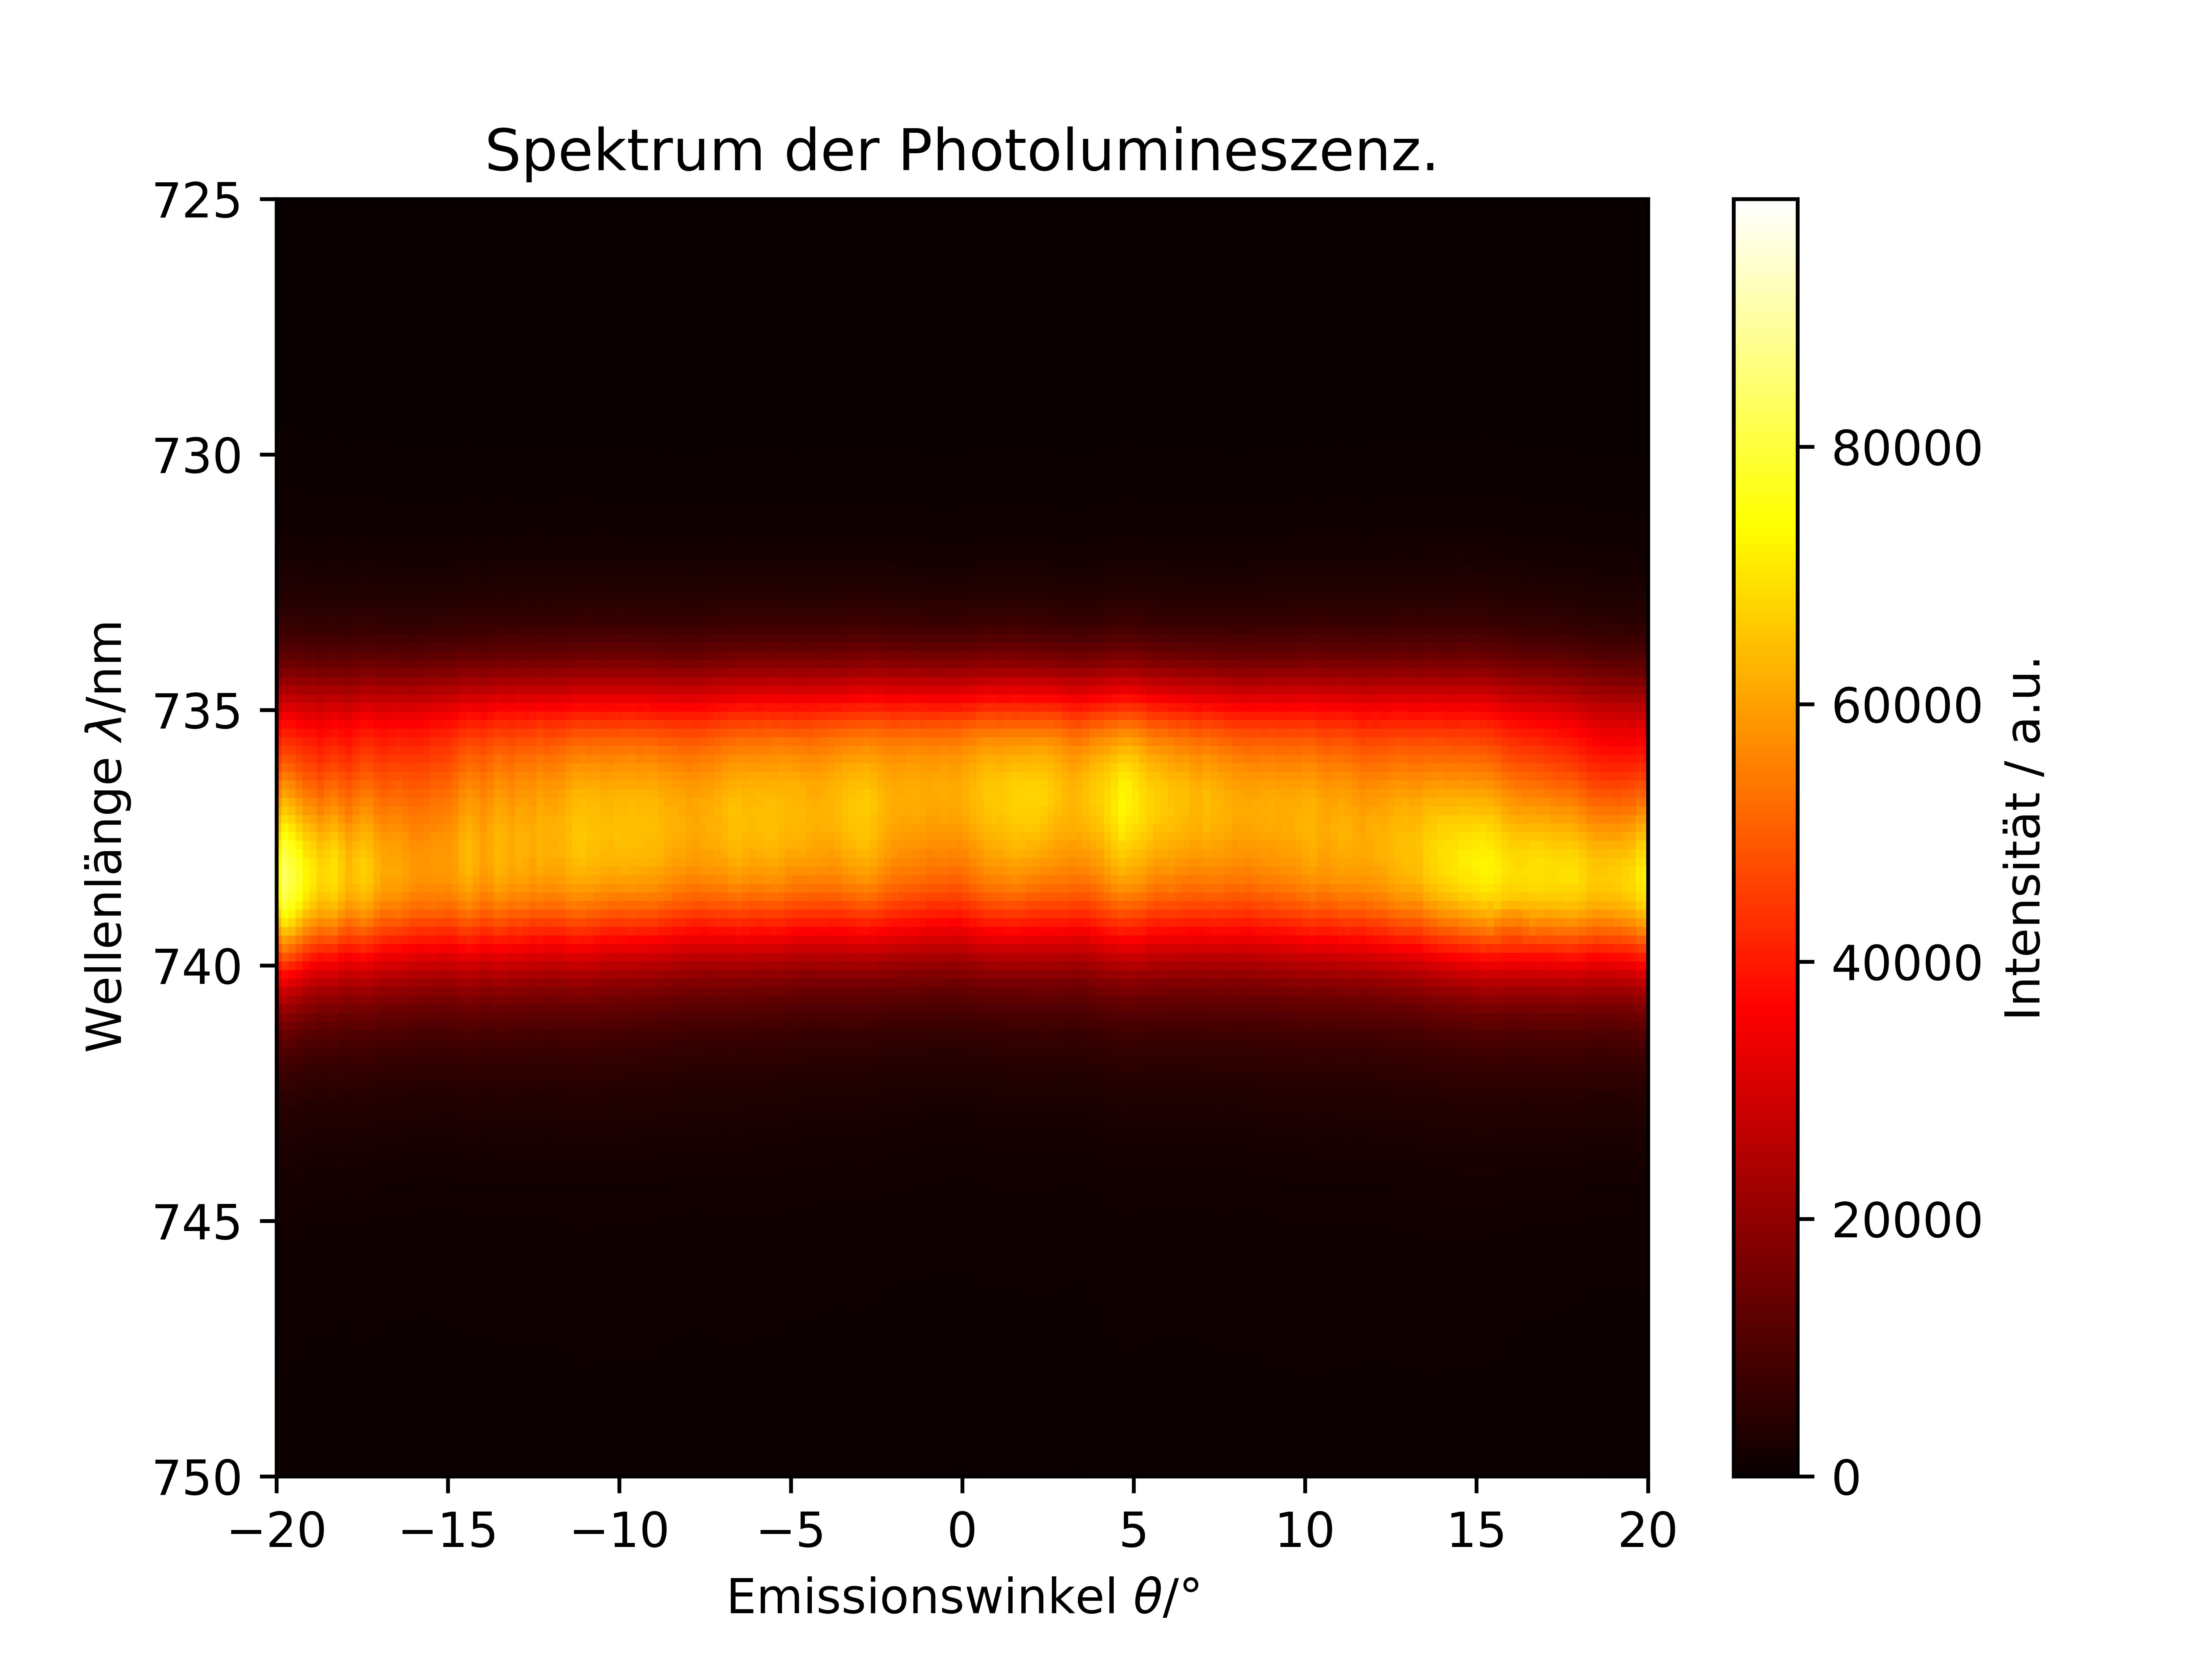
\includegraphics[scale=0.7]{./Plots/colormap__intensity_photolumineszenz_022818A 250nm 4K 2020-07-14.png}
    \caption{Darstellung des Intensitätsspektrum der Photolumineszenz.
    Die Temperatur  am Temperatursensor beträgt zum Zeitpunkt der Messung $\SI{4}{\kelvin}$. 
    Das Maximum der PL ist bei $\SI{737}{\nano\meter}$ mit einer Halbwertsbreite von ca. $\SI{5}{\nano\meter}$. 
    Je heller die Bereiche, desto mehr Intensität ist an der Stelle gemessen worden.}
    \label{fig:photo}
\end{figure}
\FloatBarrier

In Abbildung~\ref{fig:i_pn} sind die unterschiedlichen Intensitätsverläufe bei positivem und negativem
Magnetfeld im Maximum der PL und in Abhängigkeit des Emissionswinkels zu sehen.
Für die Erstellung des Graphen wurde bei der Wellenlänge $\lambda = \SI{737}{\nano\meter}$ 
über insgesamt 40 Pixel der Wellenlängenachse der CCD gemittelt.
Das entspricht einem Wellenlängenbereich von $\pm \SI{7}{\nano\meter}$ um das Maximum. 

Bei Betrachtung positiver Winkel lässt sich erkennen, dass dort die Probe mehr Licht bei negativem
Magnetfeld emittiert als bei positivem.
Eine Umkehrung des Intensitätsverlaufs ist bei Betrachtung negativer Winkel zu sehen.
Dieser Umstand deckt sich mit der vorrangestellten Theorie, da nun zirkular polarisierte Exzitonen mit dem 
umgekehrten Drehsinn entstehen und an Plasmonen mit entgegengesetzter Ausbreitungs- und Emissionsrichtung koppeln
(vgl. Abbildung~\ref{fig:zeeman}, $\sigma^- \leftrightarrow \sigma^+$).
Bei genauerer Betrachtung fällt auf, dass die beiden Graphen sich leicht links neben der $\SI{0}{\degree}$
Markierung schneiden.
Demnach muss es bei der durchgeführten Messung ($T = \SI{4}{\kelvin}$) zu äußeren Störungen gekommen sein.
\begin{figure}
    %\centering
    \begin{subfigure}{0.5\textwidth}
       %\centering
        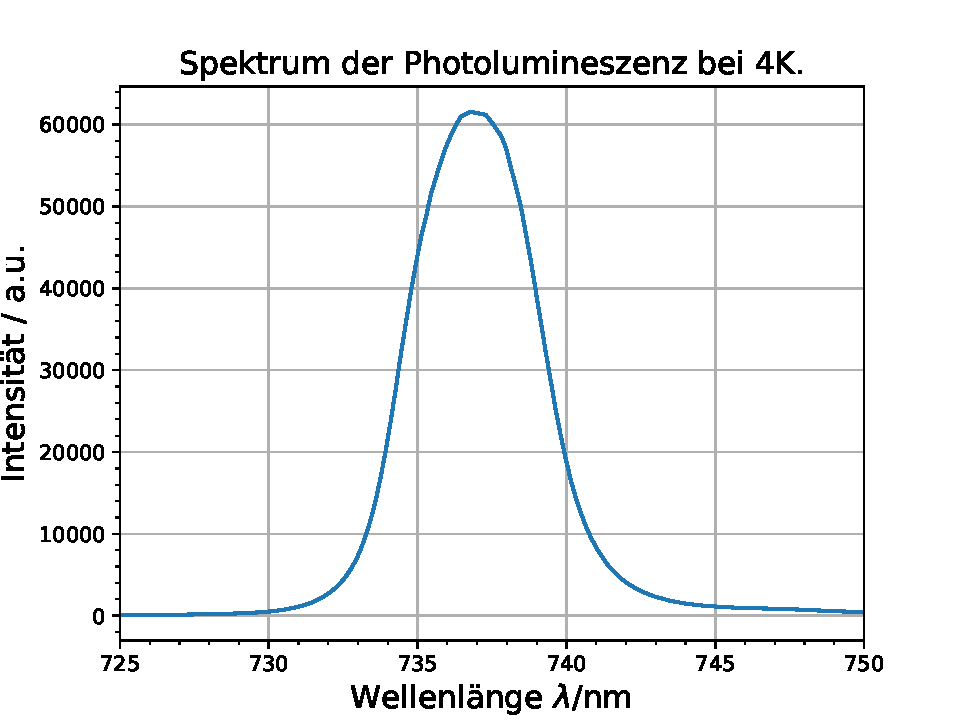
\includegraphics[scale=0.45]{./Plots/max_value_Pl_single.pdf}
        \caption{}
        \label{fig:max}
    \end{subfigure}
    \begin{subfigure}{0.5\textwidth}
        %\centering
        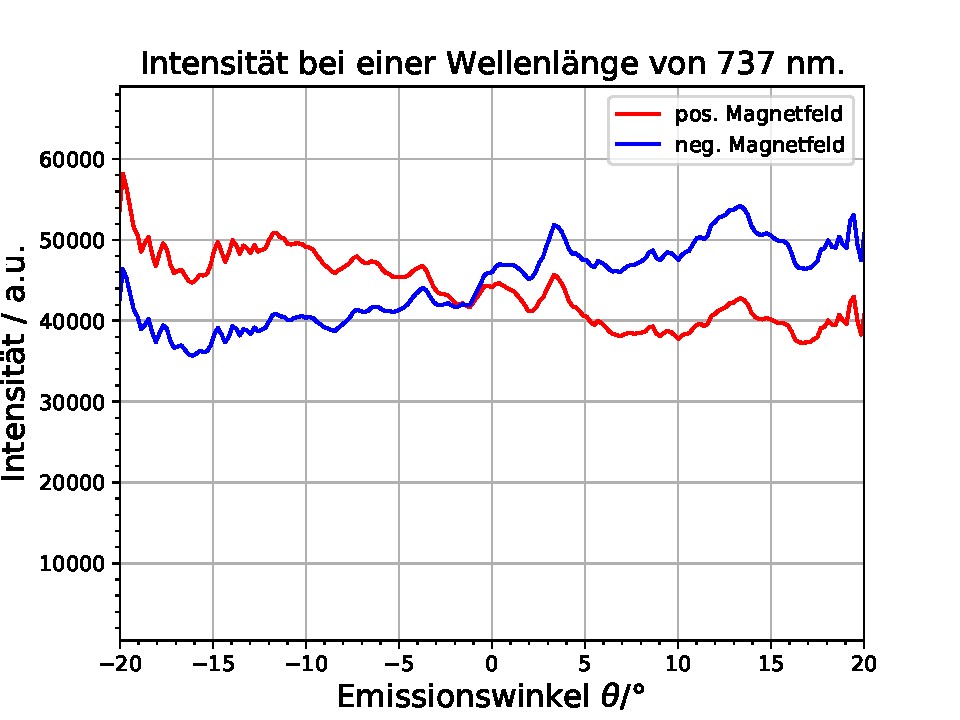
\includegraphics[scale=0.45]{./Plots/positive_and_negative_intensity_at_specific_wavelength_737_nm_022818A 250nm 4K 2020-07-14.pdf}
        \caption{}
        \label{fig:i_pn}
    \end{subfigure}
    \caption{(a) Intensitätsspektrum der PL bei $\SI{4}{\kelvin}$, gemittelt über den gesamten gemessenen 
                Winkelbereich und beide Magnetfeldrichtungen. Das Maximum der Emission liegt bei 737nm.
             (b) Darstellung des Intensitätsverlaufs der Probe beim Wechsel von positivem zu negativem Magnetfeld.
             Der Graph ist im Winkelbereich von $\SI{-20}{\degree}$ bis $\SI{20}{\degree}$ und bei einer Wellenlänge von 
             $\SI{737}{\nano\meter}$ dargestellt.
              }
    \label{fig:rho}
\end{figure}
\FloatBarrier
%%%%%%%%%%%%%%%%%%%%%%%%%%%%%%%%%%%%%%%%%%%%%%%%%%%%%%%%%%%%%%%%%%%%%%%%%%%%%%%%%%%%%%%%%%%%%%%%%%%
%\begin{figure}
%    \centering
%    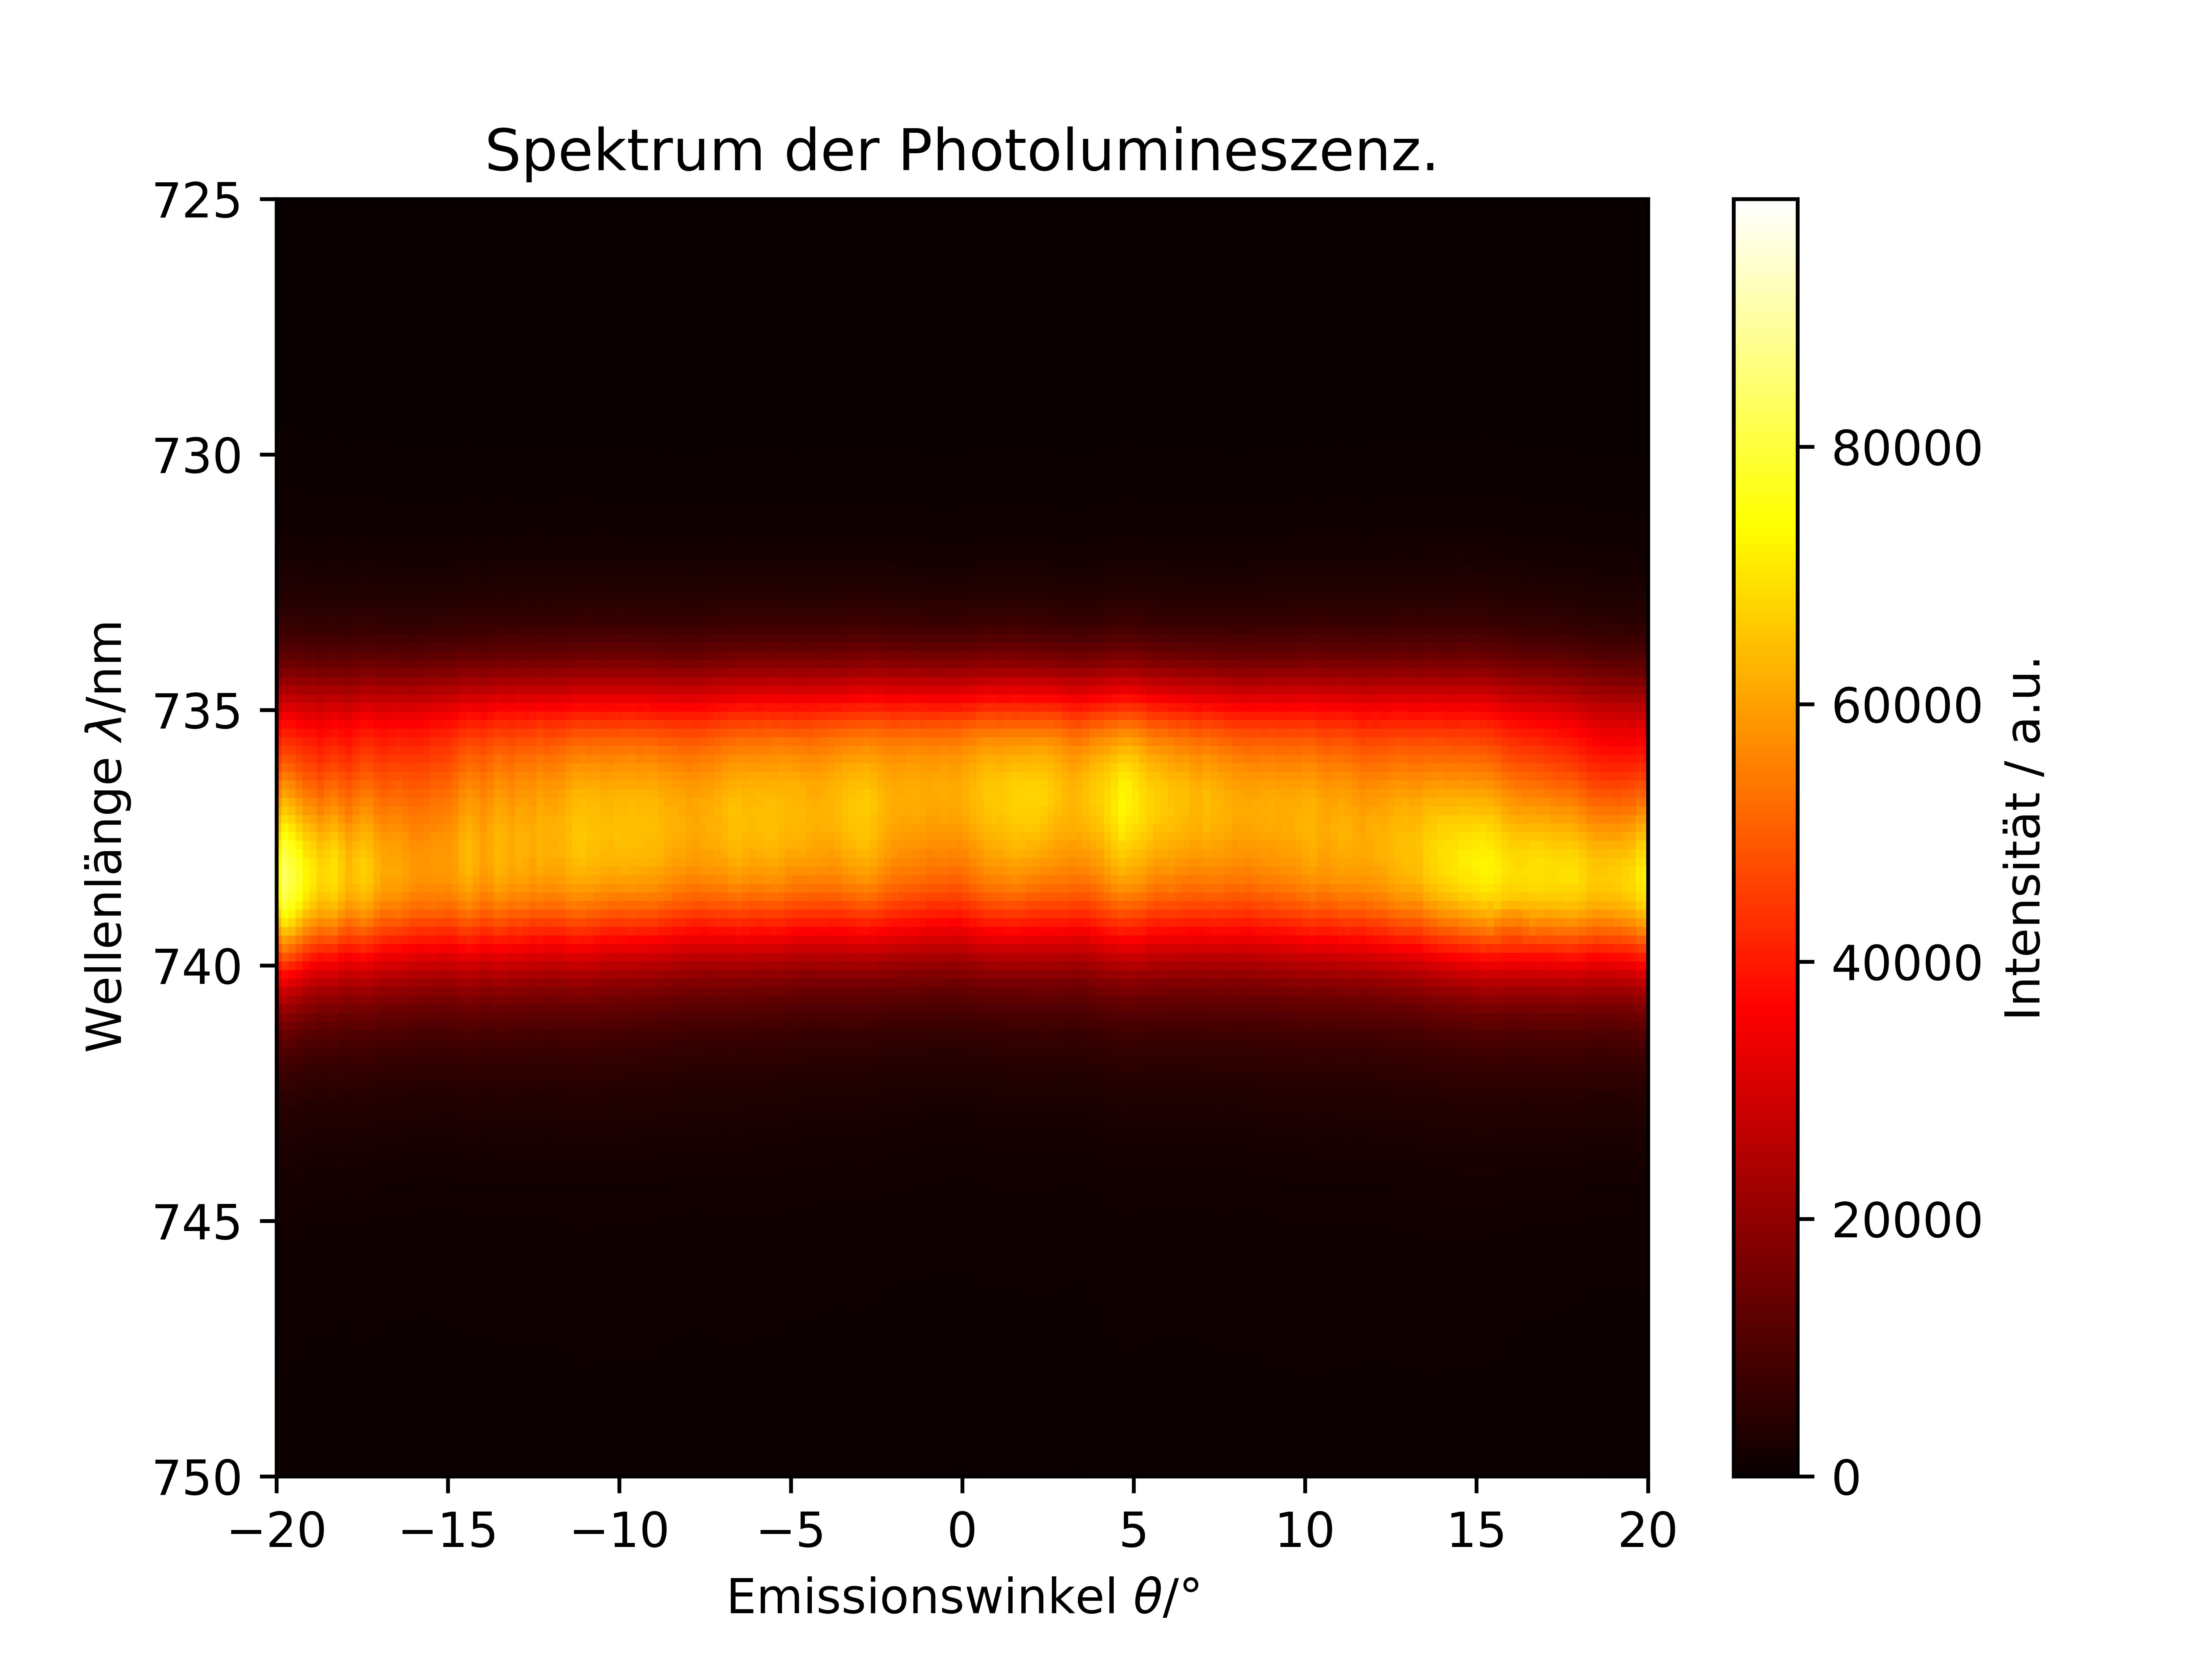
\includegraphics[scale=0.6]{./Plots/colormap__intensity_photolumineszenz_022818A 250nm 4K 2020-07-14.png}
%    \caption{Gemessene PL bei einer Temperatur von $\SI{4}{\kelvin}$. 
%    Das Maximus ist bei $\SI{737}{\nano\meter}$. 
%    Je heller die Bereiche desto mehr Intensität ist an der Stelle gemessen worden.}
%    \label{fig:photo}
%\end{figure}
%\FloatBarrier
Um die Änderung des Intensitätsverlaufs, welcher in Abbildung~\ref{fig:i_pn} zu sehen ist, zu quantifizieren,
lässt sich die Größe $\rho(\lambda,\theta)$ definieren. 
Diese wird als relative Änderung der Intensität bezeichnet.
Die relative Änderung $\rho(\lambda,\theta)$ gibt an, 
wie sehr sich die Lichtemission für einen bestimmten Winkel und Wellenlänge, bei Umpolung des Magnetfelds, ändert. 
Der Maximalwert von $\rho(\lambda,\theta)$ beträgt $1$.
Die neu definierte Größe wird mit 
\begin{equation}
    \rho = \frac{I_\text{B+} - I_\text{B-} }{ I_\text{B+} + I_\text{B-} }
\end{equation}
berechnet.
Dabei ist $I_\text{B+}$ die Intensität bei positivem Magnetfeld und $I_\text{B-}$ bei negativem Magnetfeld.

Die im Experiment bestimmte relative Änderung der Intensität $\rho(\lambda,\theta)$,
über den vollständigen Wellenlängenbereich und in Abhängigkeit des Emissionswinkels,
ist farblich in Abbildung~\ref{fig:rel_komplett} zu sehen.
Ein Teilausschnitt  ist in Abbildung~\ref{fig:rel} dargestellt.
Für beide Graphen wird ein Winkelbereich von $\pm \SI{20}{\degree}$ verwendet.
\begin{figure}
    %\centering
    \begin{subfigure}{0.50\textwidth}
        %\centering
        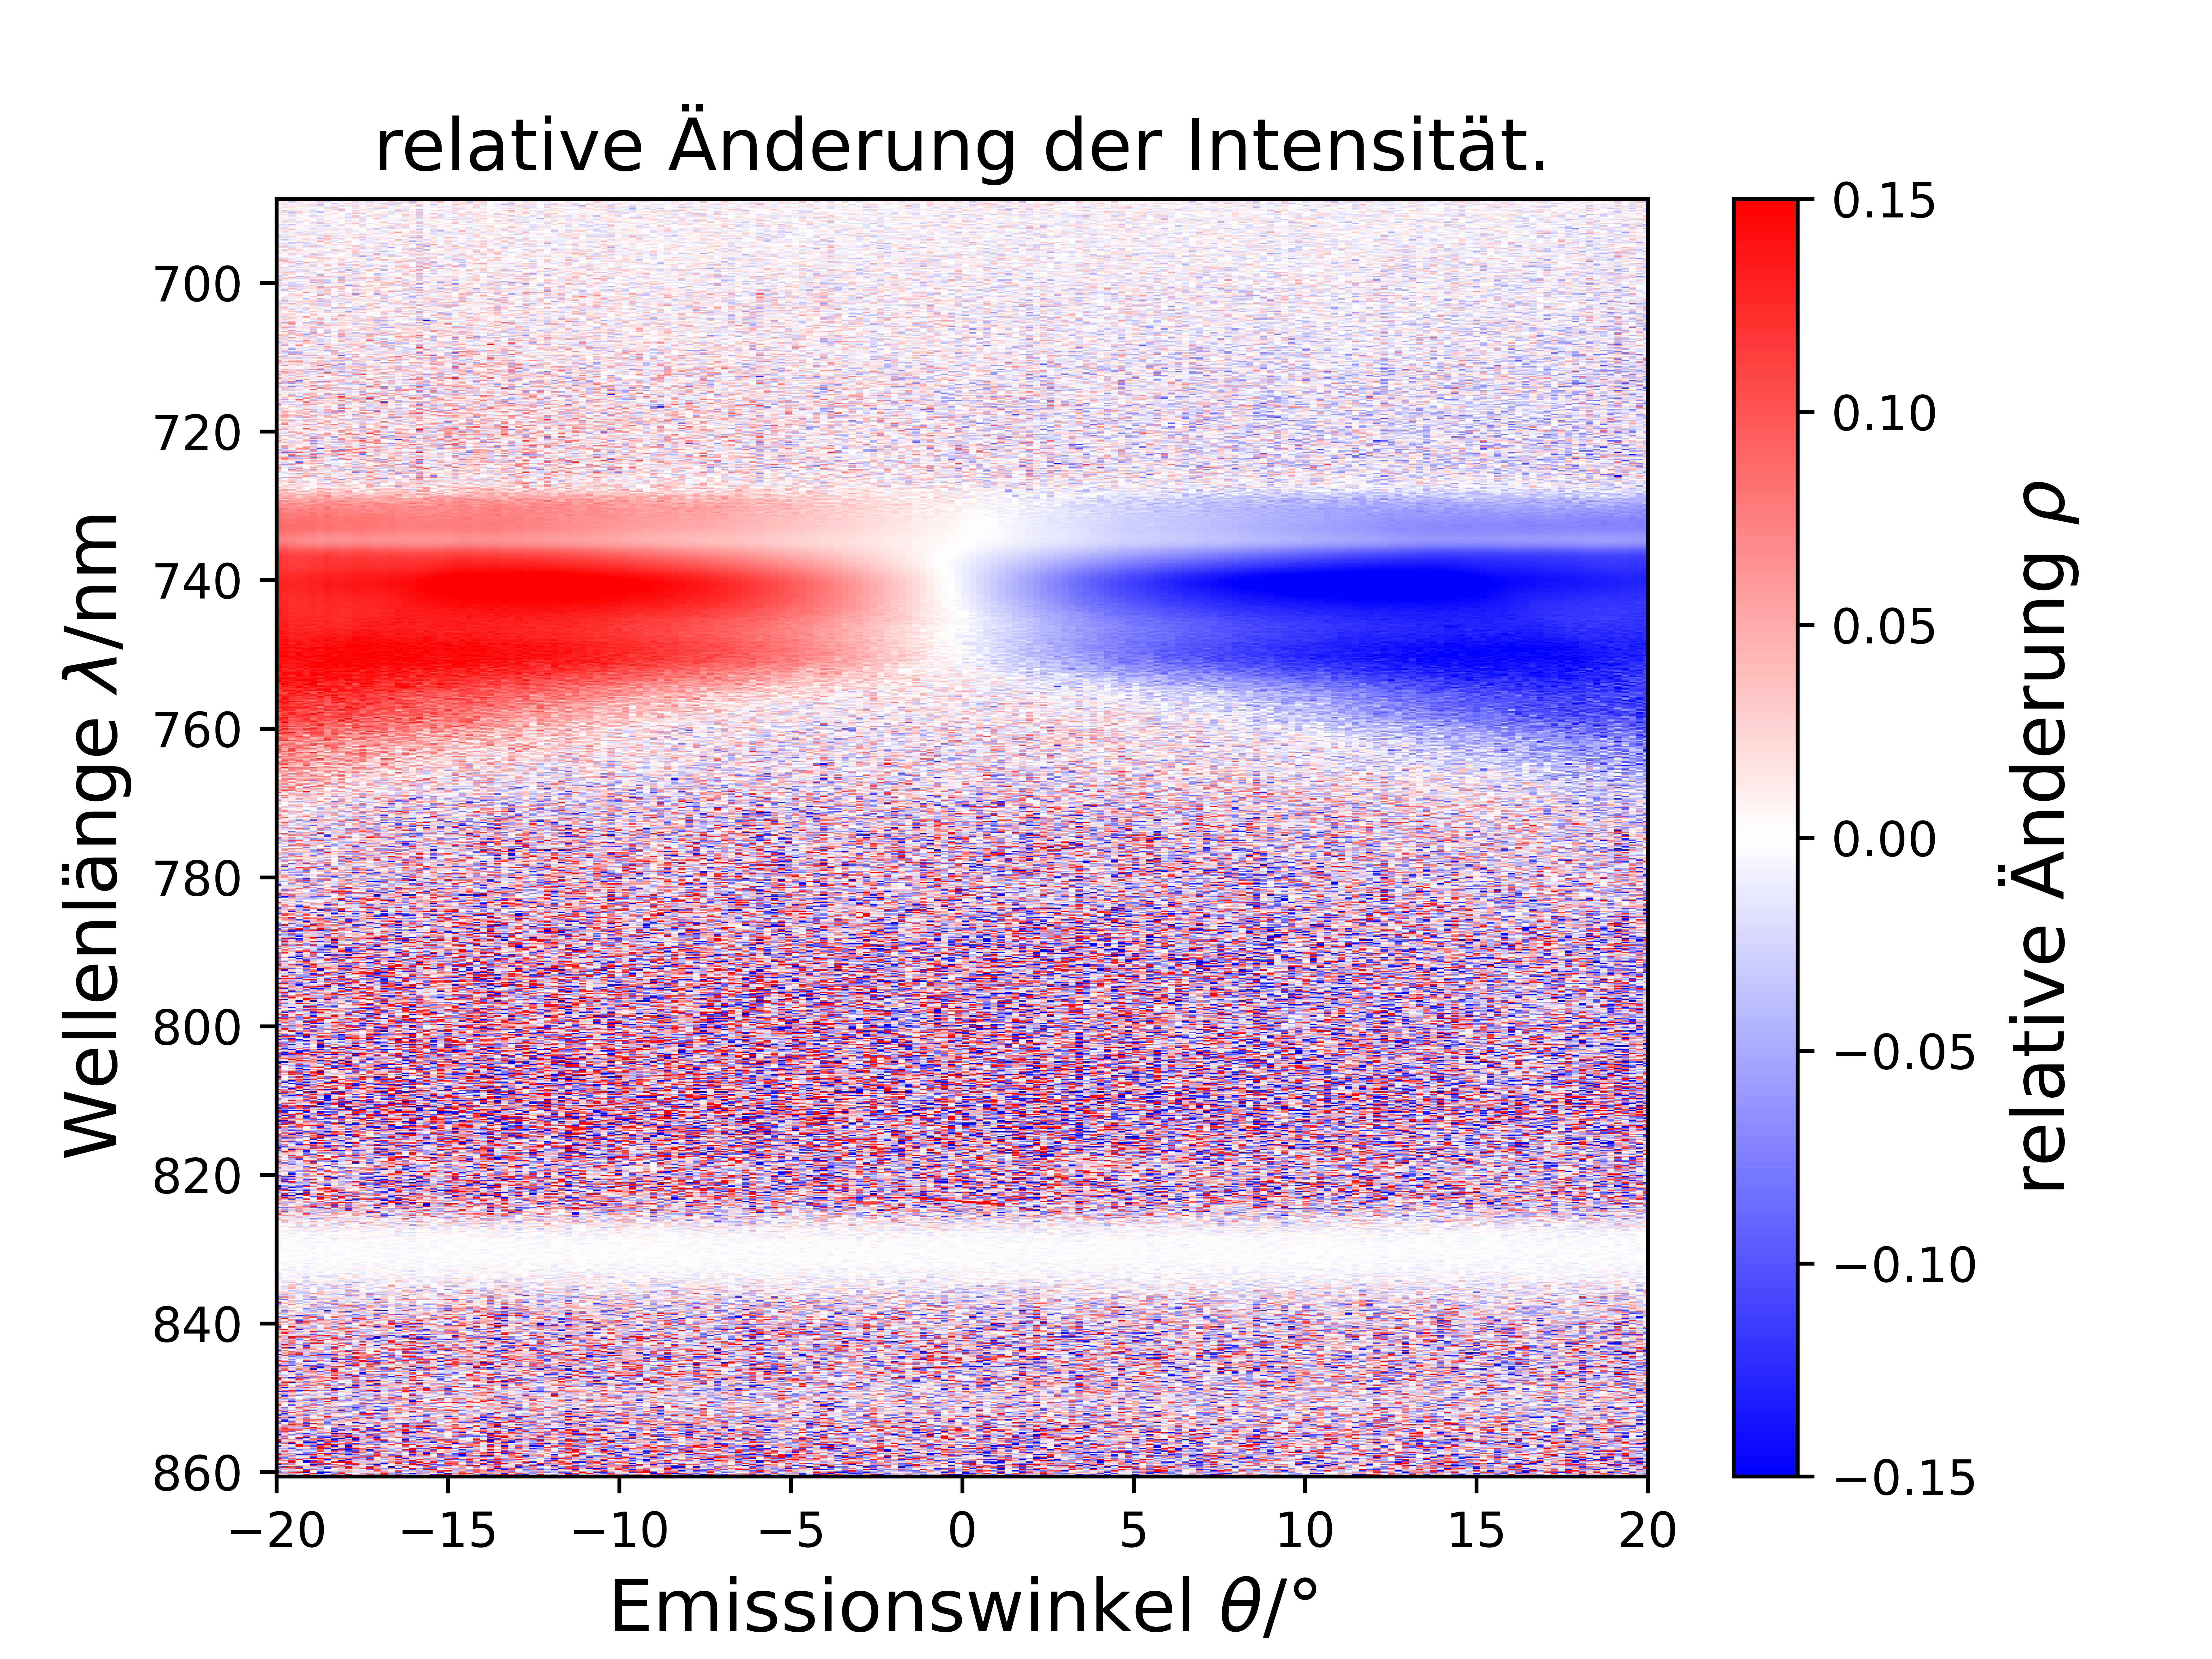
\includegraphics[scale=0.45]{./Plots/colormap_rel_change_intensity_022818A 250nm 4K 2020-07-14_komplett.png}
        %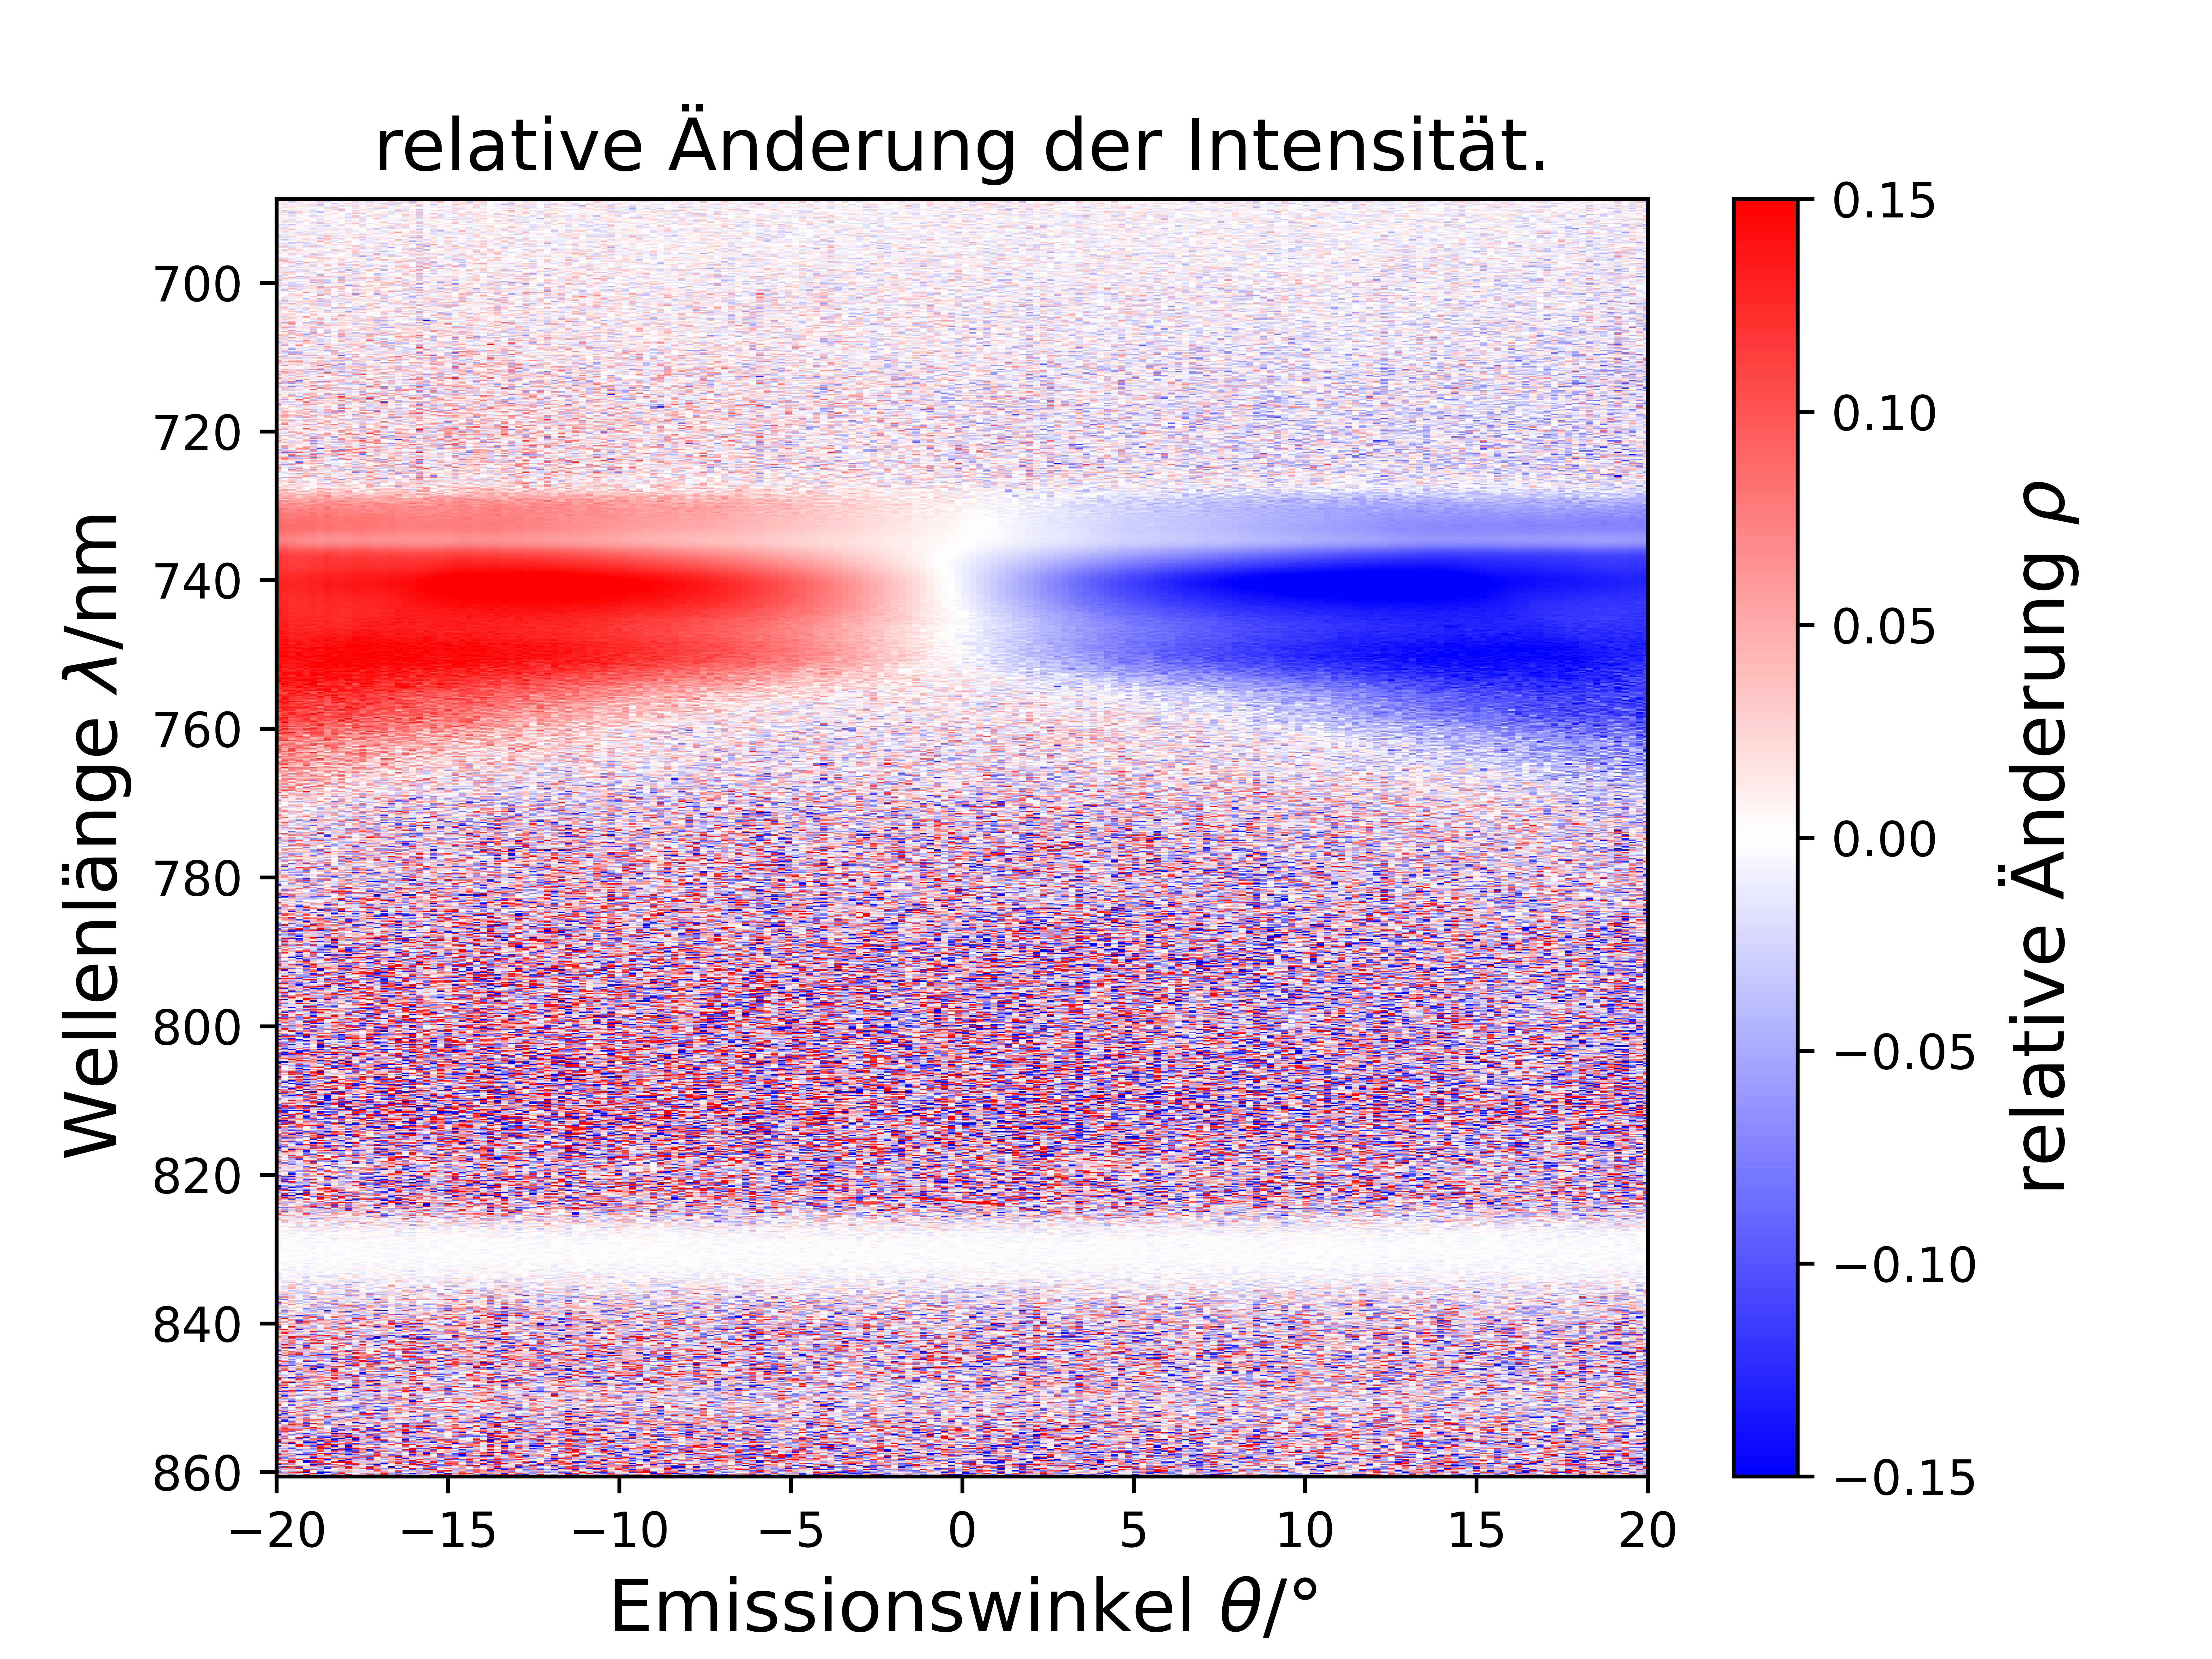
\includegraphics[scale=0.45]{./Plots/colormap_rel_change_intensity_022818A 250nm 4K 2020-07-14_komplett.pdf}
        \caption{}
        \label{fig:rel_komplett}
    \end{subfigure}
    \begin{subfigure}{0.50\textwidth}
        %\centering
        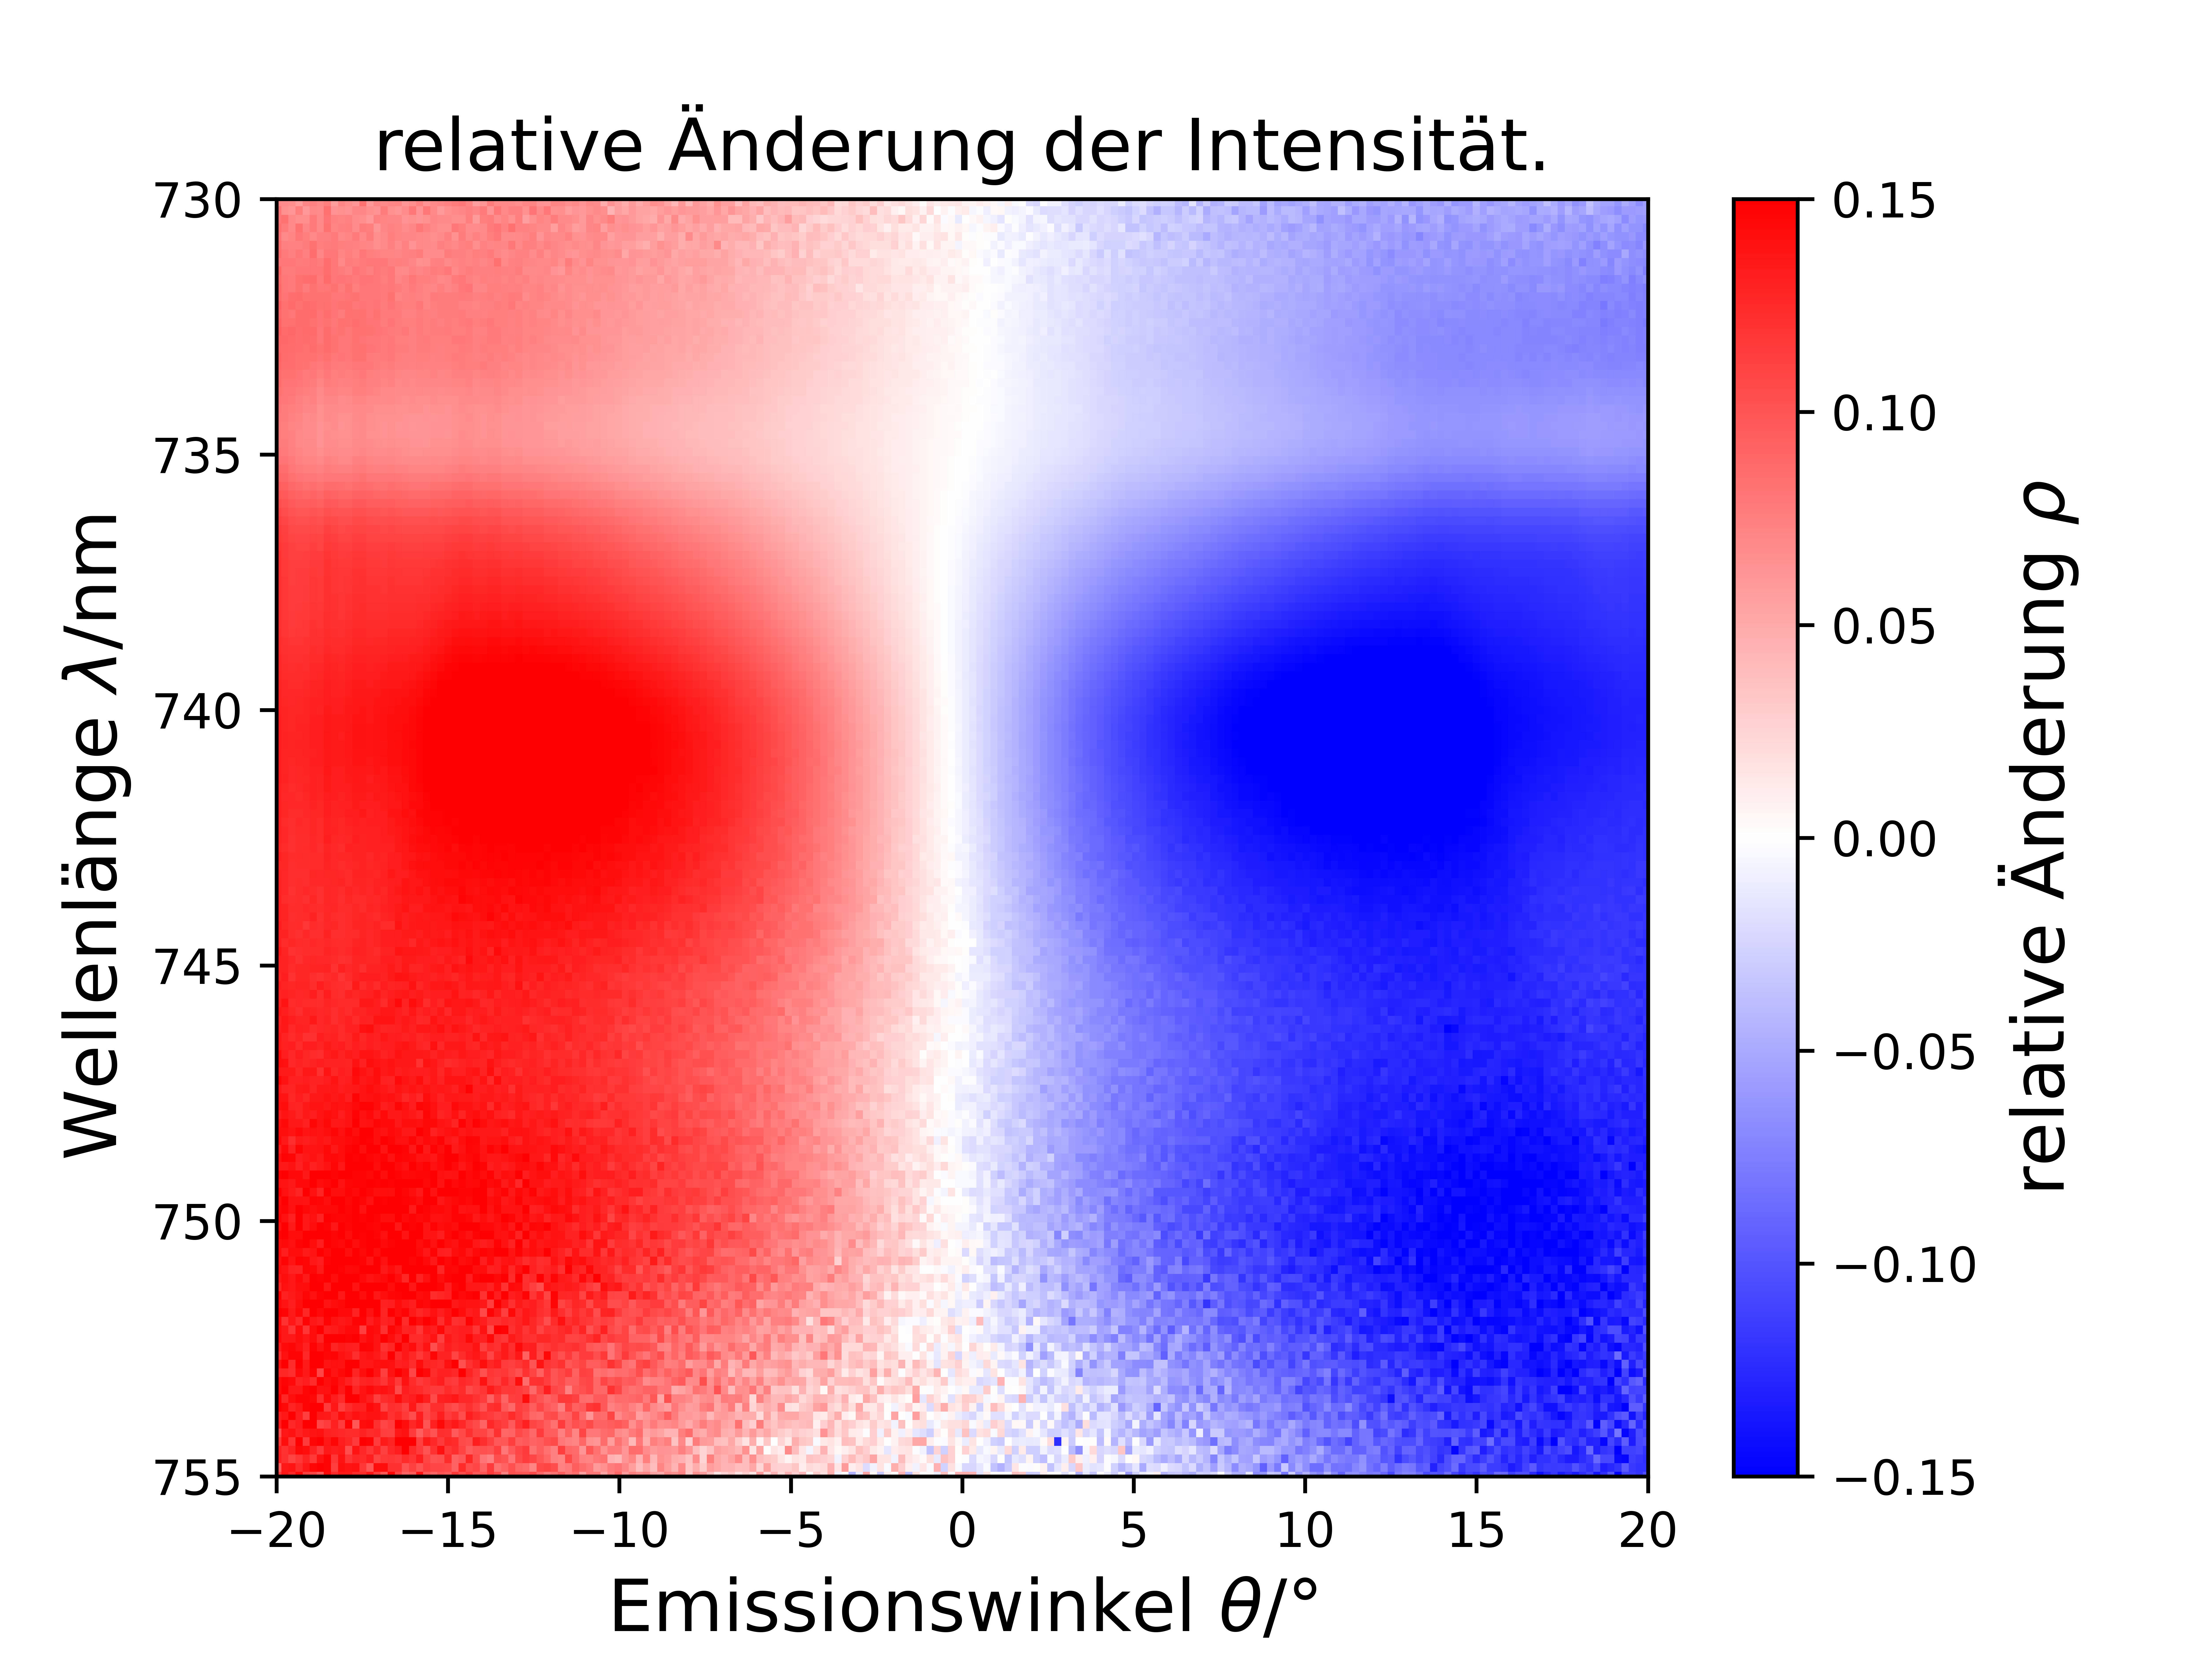
\includegraphics[scale=0.45]{./Plots/colormap_rel_change_intensity_022818A 250nm 4K 2020-07-14.png}
        %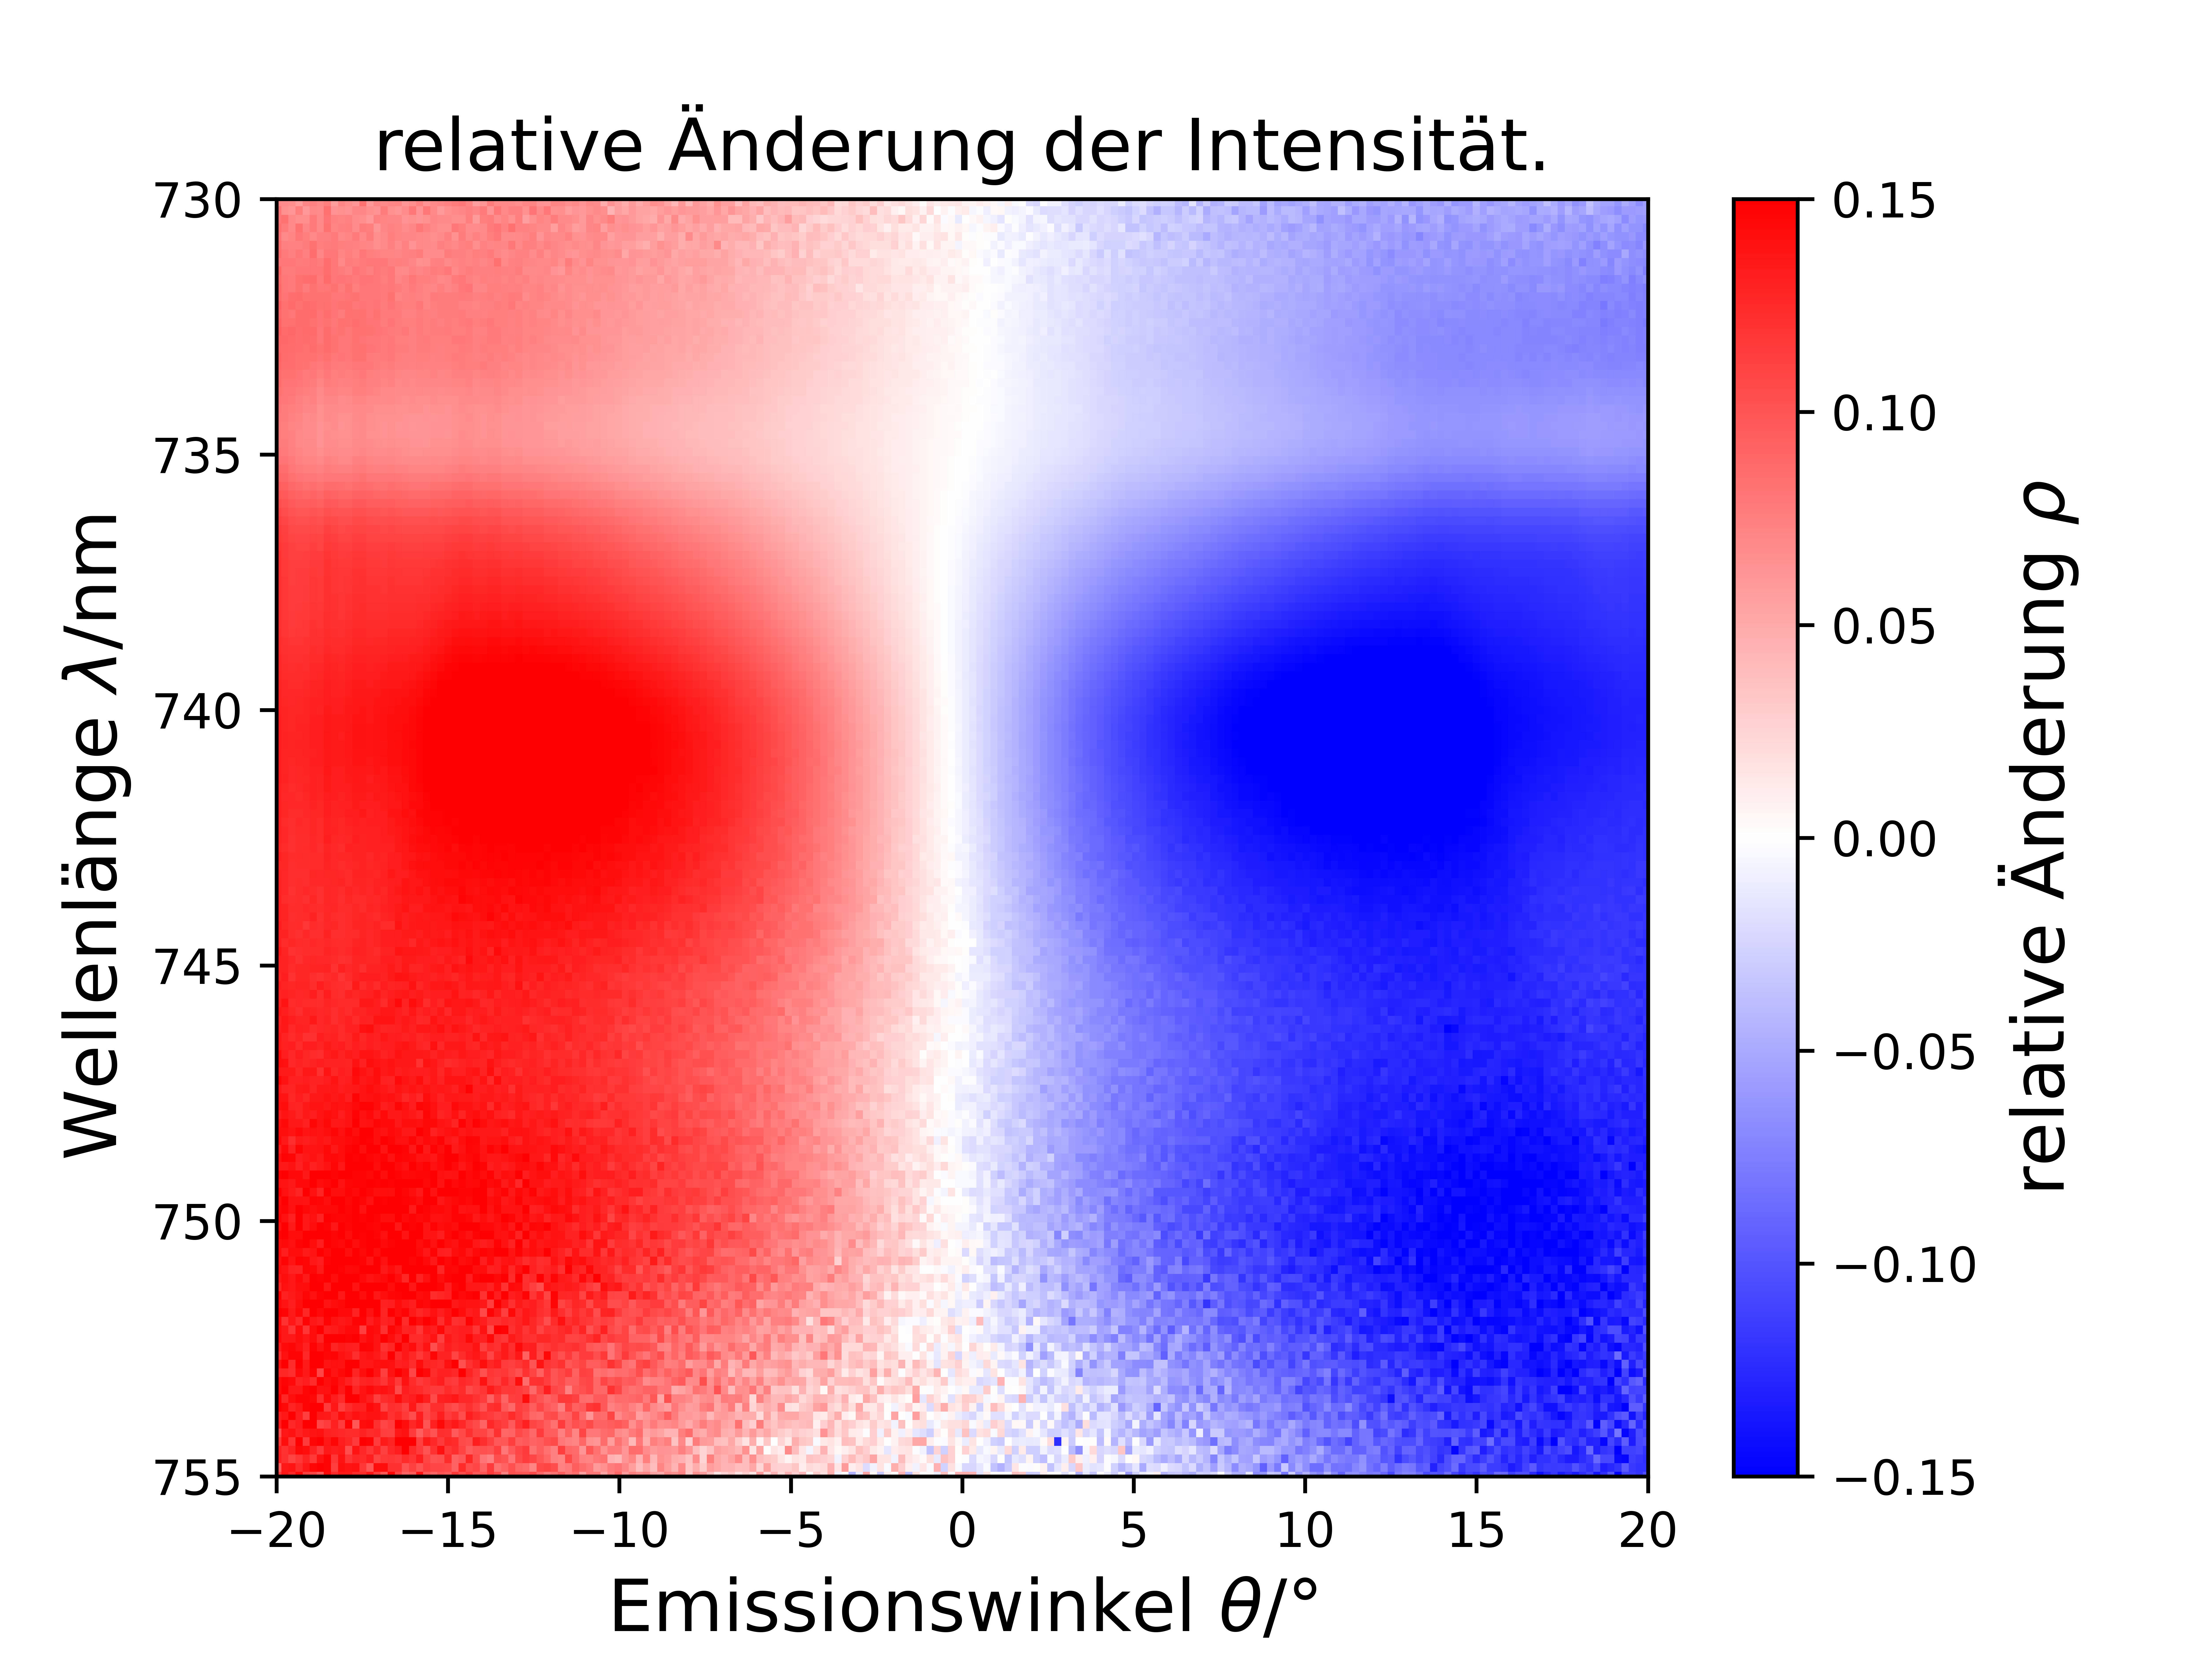
\includegraphics[scale=0.45]{./Plots/colormap_rel_change_intensity_022818A 250nm 4K 2020-07-14.eps}
        %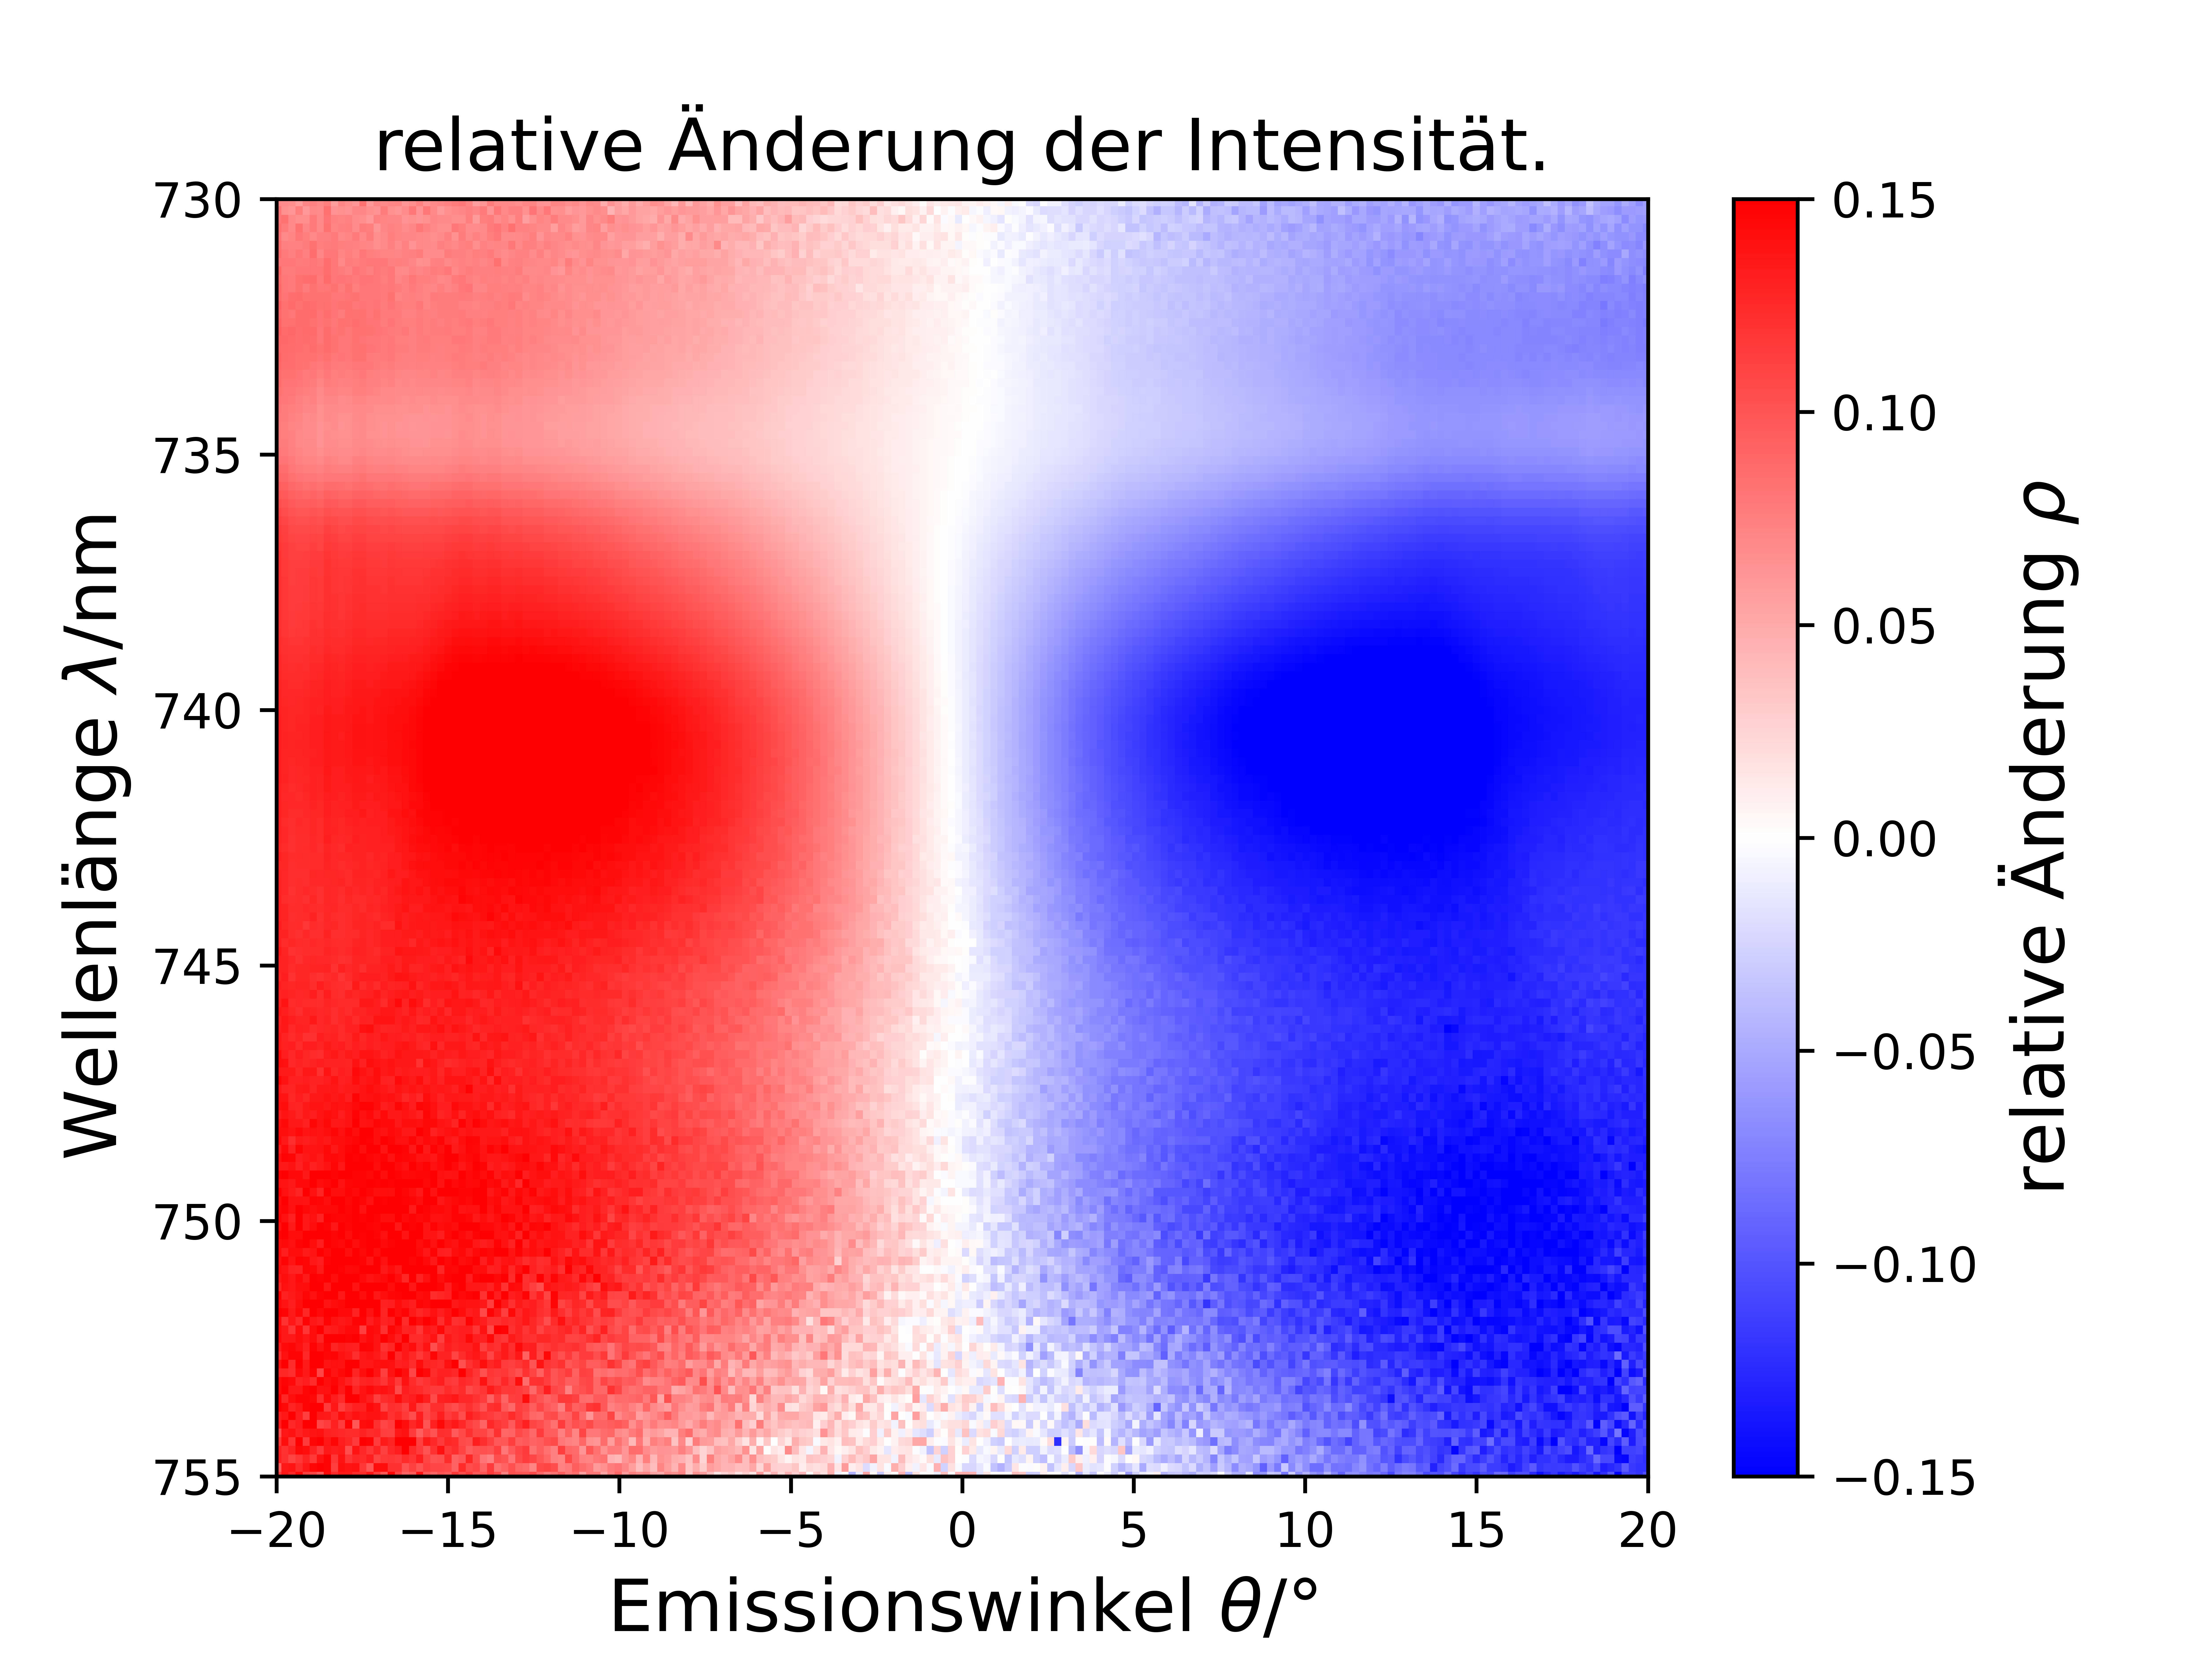
\includegraphics[scale=0.45]{./Plots/colormap_rel_change_intensity_022818A 250nm 4K 2020-07-14.pdf}
        \caption{}
        \label{fig:rel}
    \end{subfigure}
    \caption{(a) Gemessene relative Änderung der Intensität $\rho(\lambda,\theta)$, über den kompletten Wellenlängenbereich und 
    bei einer Temperatur von $\SI{4}{\kelvin}$. (b) Gemessene relative Änderung der Intensität im Bereich
    von $\SI{730}{\nano\meter}$ bis $\SI{755}{\nano\meter}$ bei einer Temperatur von $\SI{4}{\kelvin}$.}
    \label{fig:rho}
\end{figure}
\FloatBarrier
Der maximal gemessene Wert von $\rho$ im Experiment beträgt $\pm \SI{15}{\percent}$. 
Wird Abbildung~\ref{fig:rel_komplett} genauer betrachtet fällt auf, dass sich die 
gerichtete Emission im wesentlichen auf den Bereich zwischen $\SI{730}{\nano\meter}$ und $\SI{755}{\nano\meter}$
beschränkt.
Das ist im Graphen anhand der unterschiedlichen Farbintensitäten zu erkennen. 
In diesem Bereich ist für positive Emissionswinkel die relative Änderung $\rho$ negativ.
Das heißt es wird hier mehr Licht bei negativem Magnetfeld emittiert als bei positivem Magnetfeld.
Für negative Winkel ist $\rho$ positiv, was bedeutet das mehr Licht bei positivem als bei negativem Magnetfeld emittiert wird.
Der weiße Balken der im Wellenlängenbereich von ca. $\SI{825}{\nano\meter}$ bis $\SI{835}{\nano\meter}$ 
in Abbildung~\ref{fig:rel_komplett} zu sehen ist, 
hat seinen Ursprung im verwendten Substrat GaAs, 
da dieses ebenfalls zum Leuchten angeregt wird.
GaAs hat allerdings keine magnetischen Eigenschaften, 
darum entfällt die Beeinflussung durch das angelegte Magnetfeld
und es ist keine gerichtete Emission erkennbar.
Somit erscheint diese Stelle im Graphen weiß.
Der Restbereich, d.h. der Bereich ohne signifikanten Effekt, besteht aus einem statistischen Pixelrauschen der CCD.

In Abbildung~\ref{fig:rel} ist der Bereich um das Emissionsmaximum des Quantentopfes dargestellt.
Der Wellenlängenbereich liegt zwischen $\SI{730}{\nano\meter}$ und $\SI{755}{\nano\meter}$.
In der Mitte des Graphen bei $\theta = \SI{0}{\degree}$ ist ein weißer vertikaler Linienbereich zu erkennen.
Dieser Bereich entsteht, da bei einem Winkel von $\theta = \SI{0}{\degree}$ die PL genau senkrecht aus der Probe kommt
und somit keine Direktionalität aufweisen kann.
Wird der Bereich um  $\lambda = \SI{735}{\nano\meter}$ betrachtet, 
lässt sich eine schwächere Farbintensität erkennen.
Das bedeutet, dass dort die relative Änderung $\rho$ kleiner ist, sich das emittierte Licht also
weniger gut durch das angelegte Magnetfeld steuern lassen hat.
Vorhergehende Messungen haben ergeben, dass das Maximum der PL ohne Goldgitter bei 
einer Wellenlänge von $\lambda = \SI{735}{\nano\meter}$ liegt.\footnote{Die direktionale Emission ohne Goldgitter
ist sehr schwach.}
Dadurch kommt vermutlich eine Überlagerung zustande und 
es wird vermutet, dass dieses Licht aus den Randbereichen der Probe und/oder aus den Schlitzen des Goldgitters 
emittiert wird. 
Somit sinkt insgesamt die Direktionalität in diesem Bereich.

Die Oszillationen entlang der Wellenlängenachse (Periode etwa $\SI{10}{\nano\meter}$) 
ergeben sich aus der Interferenz von Strahlung, die direkt die Probe verlässt und solcher, 
die zuerst am Substrat reflektiert wurde und dann die Probe in gleicher Richtung verlässt. 
Dieser Effekt tritt ebenfalls auf, 
wenn sich kein Goldgitter auf der Probe befindet und ist deutlich schwächer als der plasmonische Effekt.\cite{lars}
Im Wellenlängenbereich zwischen $\SI{738}{\nano\meter}$ und $\SI{740}{\nano\meter}$ lässt sich durch die hohe
Farbintensität erkennen, dass hier die beste Steuerung der Lichtemission durch das Magnetfeld gelungen ist.

Wird die relative Änderung der Intensität $\rho$ in Abhängigkeit des Winkelbereichs und bei 
konstanter Wellenlänge von $\lambda = \SI{737}{\nano\meter}$
betrachtet, ergibt sich der Graph in Abbildung~\ref{fig:dir}.
Es fällt auf, dass 
der Graph von $\rho$, bis auf eine kleine Abweichung am Nullpunkt,
antisymmetrisch ist.
Dieser Befund deckt sich mit den theoretischen Betrachtungen 
und den experimentellen Befunden an einer ähnlichen Probe \cite{felix}.

Bei genauerer Analyse des Graphen der Direktionalität lässt sich erkennen, dass bis ca. $\theta = \pm \SI{5}{\degree}$
die Steigung von $\rho$ linear ist.
Wird dieser Wert über- bzw. unterschritten geht der Graph in eine Krümmung über, die bei $\theta = \pm \SI{13,5}{\degree}$
ihr Maximum besitzt. 
Der dazugehörige Maximalwert beträgt $\rho = \SI{11,5}{\percent}$. 
Hinter dem Maximum schwächt sich die Direktionalität ab.

%\begin{figure}
%    \centering
%    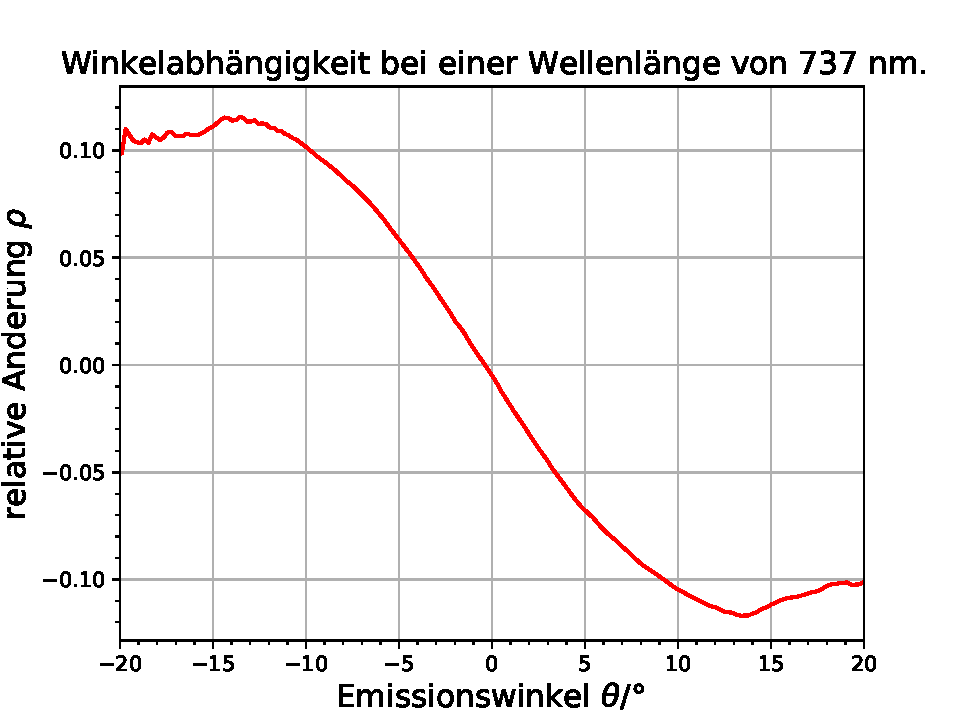
\includegraphics[scale=0.7]{./Plots/rho_at_specific_wavelength_737_nm_022818A 250nm 4K 2020-07-14.pdf}
%    \caption{Gemessene Direktionalität $\rho$ im Maximum der Photolumineszenz.
%    Der maximale Wert der im Experiment gemessen Direktionalität ist hier $\rho = \SI{11,5}{\percent}$.}
%    \label{fig:dir}
%\end{figure}
%\FloatBarrier
Da bereits in mehreren Experimenten unabhängig von dieser Arbeit bestätigt wurde, dass der Graph
der Direktionalität antisymmetrisch sein muss, wird nun nur noch der antisymmetrische Anteil von $\rho$ betrachtet.  
Dazu wird der Direktionalitätsfaktor $C$, kurz Direktionalität, eingeführt. 

Es gilt 
\begin{equation}
    C= \frac{\rho(-\theta)-\rho(\theta)}{2}.
    \label{eq:C} 
\end{equation}

Vergleichend zu Abbildung~\ref{fig:dir} ist der Verlauf der Direktionalität in Abbildung~\ref{fig:dir_kor} zu sehen.
Bei der Betrachtung der beiden Graphen lässt sich erkennen, dass diese nur sehr geringfügig voneinander 
abweichen, das spricht für eine gewisse Genauigkeit der Messung.
\begin{figure}
    %\centering
    \begin{subfigure}{0.50\textwidth}
        %\centering
        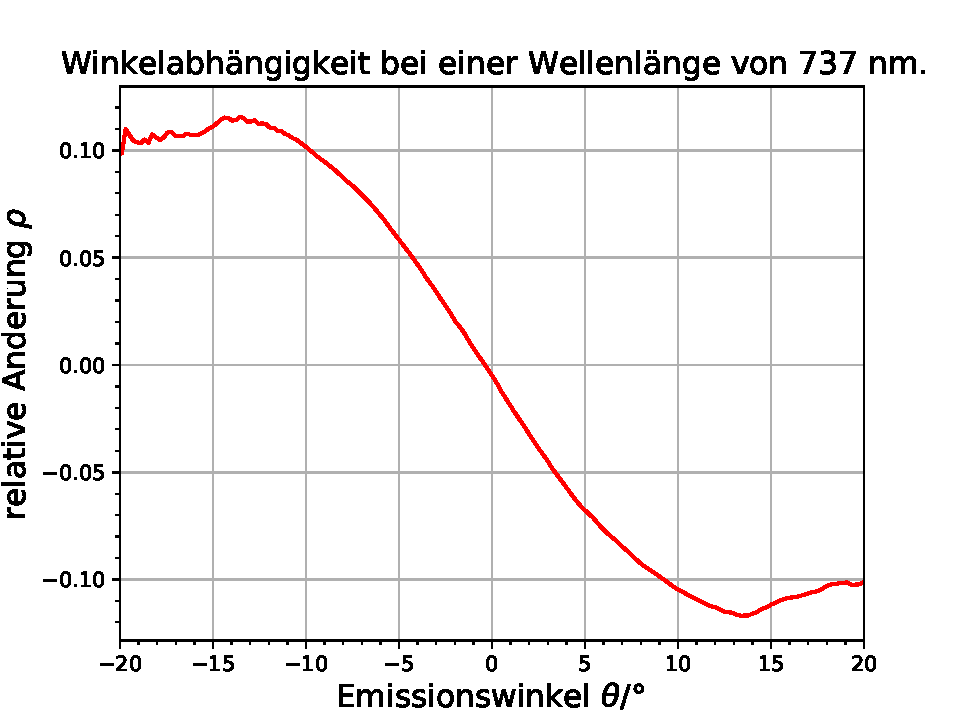
\includegraphics[scale=0.45]{./Plots/rho_at_specific_wavelength_737_nm_022818A 250nm 4K 2020-07-14.pdf}
        \caption{}
        \label{fig:dir}
    \end{subfigure}
    \begin{subfigure}{0.50\textwidth}
        %\centering
        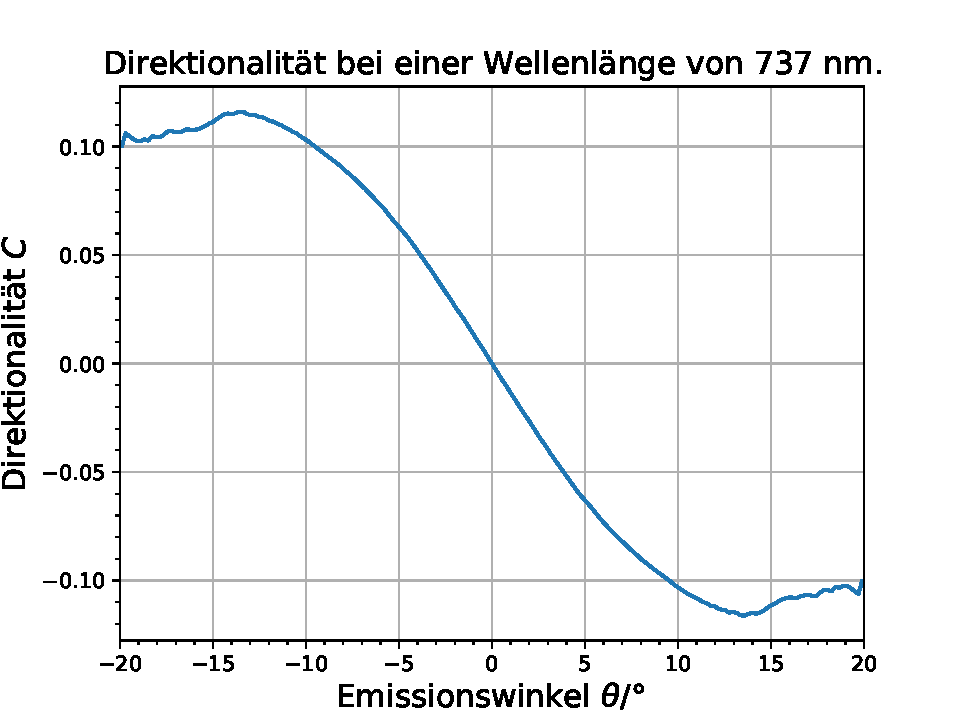
\includegraphics[scale=0.45]{./Plots/rho_at_specific_wavelength_737_nm_022818A 250nm 4K 2020-07-14_korrigiert.pdf}
        \caption{}
        \label{fig:dir_kor}
    \end{subfigure}
    \caption{(a) Gemessene Direktionalität $\rho$ im Maximum der Photolumineszenz.
    Der maximale Wert der im Experiment gemessen Direktionalität ist hier $\rho = \SI{11,5}{\percent}$.
     (b) Darstellung des Verlaufs der Direktionalität $C$.
     Die Direktionalität $C$ bei $\SI{737}{\nano\meter}$ unterscheidet sich von $\rho$ indem sie nur die antisymmetrischen
     Anteile berücksichtigt. Der Graph von $\rho$ unterscheidet sich nur geringfügig von dem hier 
     abgebildeten Verlauf. Dies spricht für eine gewisse Genauigkeit der Messungen im Experiment.}
    \label{fig:dir_merged}
\end{figure}
\FloatBarrier 
%\begin{figure}
%    \centering
%    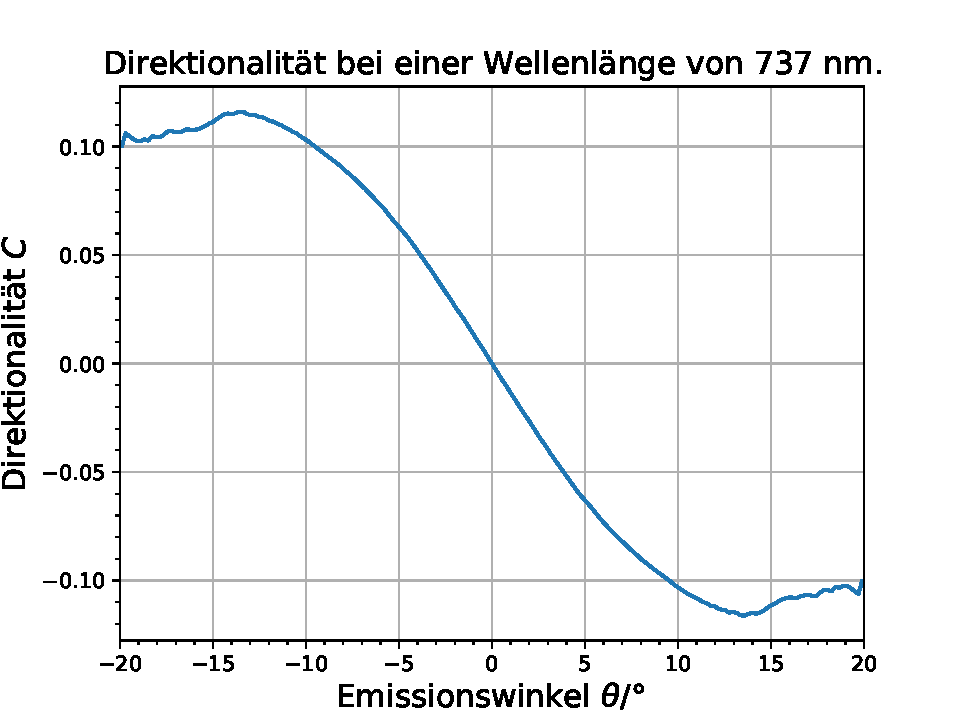
\includegraphics[scale=0.7]{./Plots/rho_at_specific_wavelength_737_nm_022818A 250nm 4K 2020-07-14_korrigiert.pdf}
%    \caption{Darstellung des Verlaufs der Direktionalität $C$.
%     Die Direktionalität $C$ unterscheidet sich von $\rho$ indem sie nur die antisymmetrischen
%     Anteile berücksichtigt. Der Graph von $\rho$ unterscheidet sich nur geringfügig von dem hier 
%     abgebildeten Verlauf, dies spricht für eine gewisse Genauigkeit der Messungen im Experiment. }
%    \label{fig:dir_kor}
%\end{figure}
%\FloatBarrier

\section{Temperaturabhängigkeit der Direktionalität}~\label{sec:Temperatur Abhaengigkeit der Direktionalitaet}
Im folgenden Abschnitt der Arbeit wird die Temperaturabhängigkeit der im Experiment
beobachteten Direktionalität $C$ diskutiert und wesentliche Aspekte erläutert.

Die Direktionalität der Probe wurde über einen Temperaturbereich von $ \Delta T =\SI{41}{\kelvin} $ gemessen.
Die kleinste eingestellte Temperatur ist dabei $T =\SI{4}{\kelvin}$ gewesen, die größte 
$T =\SI{45}{\kelvin}$.
Es sind insgesamt 11 temperaturabhängige Messungen entstanden.

Die Wellenlänge, bei der alle nachfolgenden Graphen betrachtet werden ist, \\$\lambda =\SI{738}{\nano\meter}$,
da dies etwa dem über alle Temperaturen gemittelten Maximum der Photolumineszenz entspricht.
%Im Abbildung~\ref{fig:int_temp} sind die Intensitätsmaxima bei den unterschiedlichen Temperaturen zu sehen.
%\begin{figure}
%    \centering
%    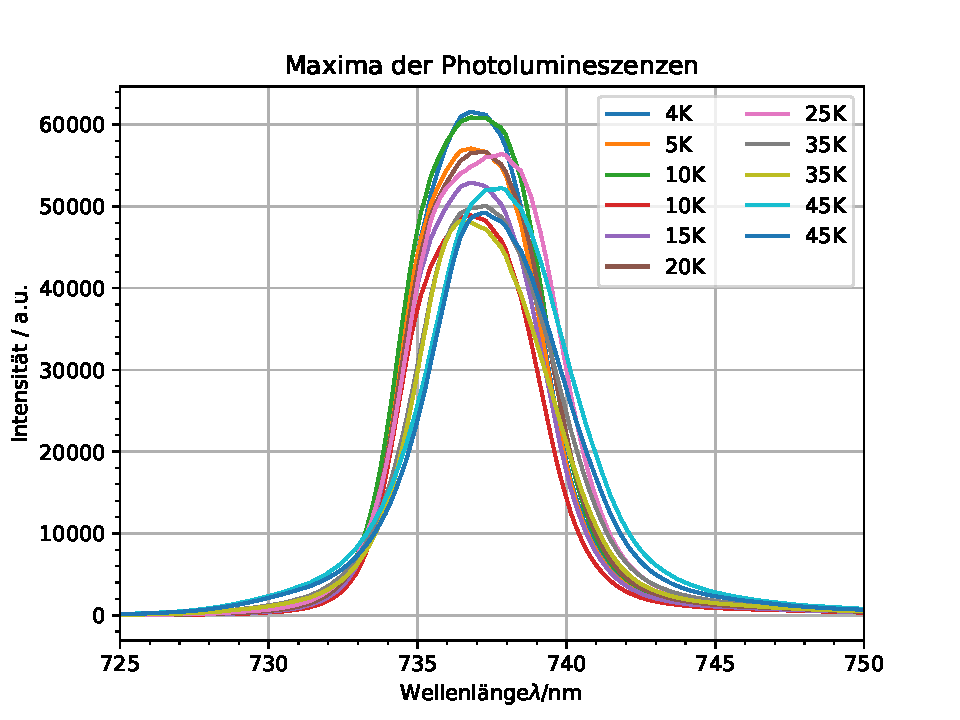
\includegraphics[scale=0.7]{./Plots/max_value_Pl_alle.pdf}
%    \caption{Darstellung der Intensitätsmaxima bei unterschiedlichen Temperaturen.
%    Das gemittelte Maxima ist bei $\lambda =\SI{737,7}{\nano\meter}$.}
%    \label{fig:int_temp}
%\end{figure}
%\FloatBarrier 

In Abbildung~\ref{fig:temp_all_nach} sind die winkelabhängigen Direktionalitäten für die untersuchten Temperaturen
bei konstanter Wellenlänge abgebildet.
%\begin{figure}
%    \centering
%    \begin{subfigure}{0.55\textwidth}
%       %\centering
%        \includegraphics[scale=0.45]{./Plots/Temperaturabhaengigkeit_rho_at_738_nm_4K5K10K10K15K20K25K35K35K45K45K_vorher.pdf}
%        \caption{Darstellung der Direktionalität $\rho$ bei konstanter Wellenlänge und  unterschiedlichen Temperaturen.
%         Die Wellenlänge beträgt $\lambda =\SI{738}{\nano\meter}$.}
%        \label{fig:temp_all_vor}
%    \end{subfigure}
%    \begin{subfigure}{0.55\textwidth}
%        %\centering
%        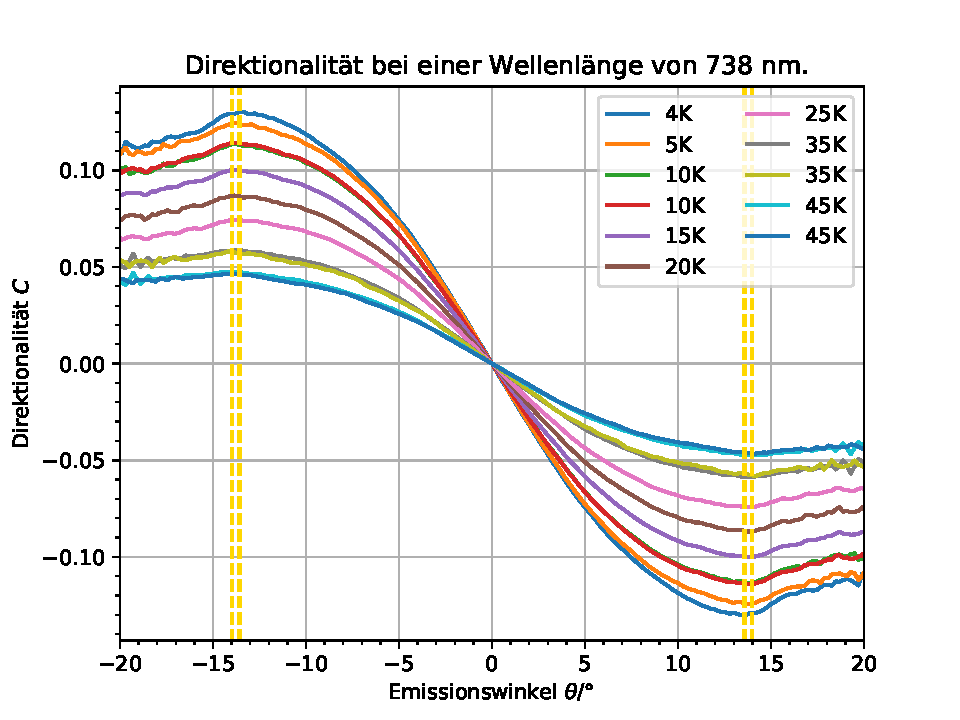
\includegraphics[scale=0.45]{./Plots/Temperaturabhaengigkeit_rho_at_738_nm_4K5K10K10K15K20K25K35K35K45K45K_korrigiert.pdf}
%        \caption{Darstellung der Direktionalität $C$ bei konstanter Wellenlänge und  unterschiedlichen Temperaturen.
%         Die Wellenlänge beträgt $\lambda =\SI{738}{\nano\meter}$.}
%        \label{fig:temp_all_nach}
%    \end{subfigure}
%    \caption{In der linken Abbildung ist die Direktionalität $\rho$ zu sehen, in der rechten der Direktionalitätsfaktor $C$.}
%    \label{fig:temp_verlauf}
%\end{figure}
%\FloatBarrier
%TODO fix der zeichnungen
\newpage %lol
\begin{figure}
    \centering
    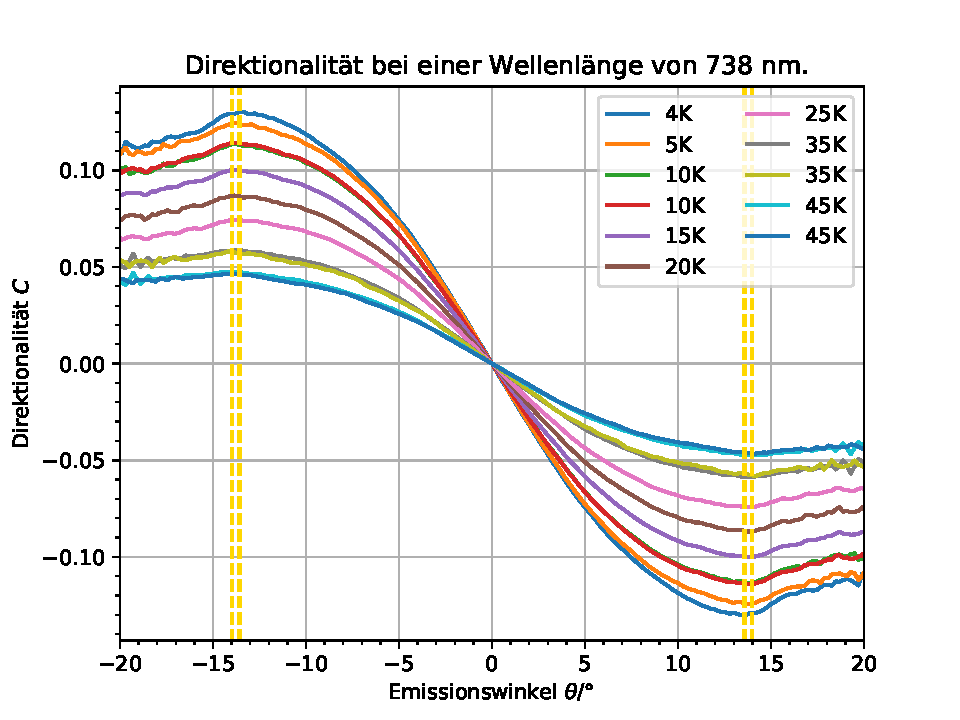
\includegraphics[scale=0.7]{./Plots/Temperaturabhaengigkeit_rho_at_738_nm_4K5K10K10K15K20K25K35K35K45K45K_korrigiert.pdf}
    \caption{Darstellung der Direktionalität $C$ bei unterschiedlichen Temperaturen und konstanter Wellenlänge 
    von $\lambda =\SI{738}{\nano\meter}$. 
    Der gemessene Temperaturbereich geht von \SI{4}{\kelvin} bis \SI{45}{\kelvin}.
    Es ist erkennbar, dass mit steigender Temperatur die gemessene Direktionalität $C$ immer mehr sinkt.}
    \label{fig:temp_all_nach}
\end{figure}
\FloatBarrier

Die gelb gestrichelten Linien in Abbildung~\ref{fig:temp_all_nach} markieren die Bereiche 
in denen die Maxima der Direktionalitäten
bei unterschiedlichen Temperaturen liegen.
Der Winkelbereich, in denen sich die Maxima befinden, erstreckt sich von  $\theta = \pm \SI{13,58}{\degree} 
$ bis $ \theta = \pm \SI{13,98}{\degree}$.
%In Tabelle~\ref{tab:rc} ist ein Vergleich der Werte von $\rho$ und $C$ zu dargestellt.  
Bei Betrachtung der Messungen mit gleicher Temperatur (z.B. $\SI{10}{\kelvin}$) 
überlappen sich die Verläufe von $C$ sehr gut.
Bei ungleichen Temperaturen lässt sich ein deutlicher Unterschied erkennen.
Graphisch entsteht eine sichtbare Abflachung und Verringerung des Verlaufs von $C$.
Das bedeutet, dass die Direktionalität mit der Temperatur sinkt.
Sehr deutlich ist das bei Betrachtung der beiden Randwerte 
der Temperaturen $T = \SI{4}{\kelvin}$ und $ T = \SI{45}{\kelvin}$ zu sehen.
Die Direktionalität fällt hier von $C= \SI{13}{\percent}$ auf $C = \SI{4,8}{\percent}$ ab.

Werden die jeweiligen Maximalwerte der Direktionalität $C$ in Abhängigkeit
der Temperatur dargestellt, entsteht der Graph in Abbildung~\ref{fig:fit}.
Alleine anhand des Graphen lässt sich eine Temperaturabhängigkeit der Direktionalität
feststellen.
Mit steigender Temperatur sinkt die Direktionalität.
Der Zusammenhang, der zwischen der Direktionalität und der Temperatur besteht, lässt sich 
quantifizieren.
\newpage %lol
\begin{figure}
    \centering
    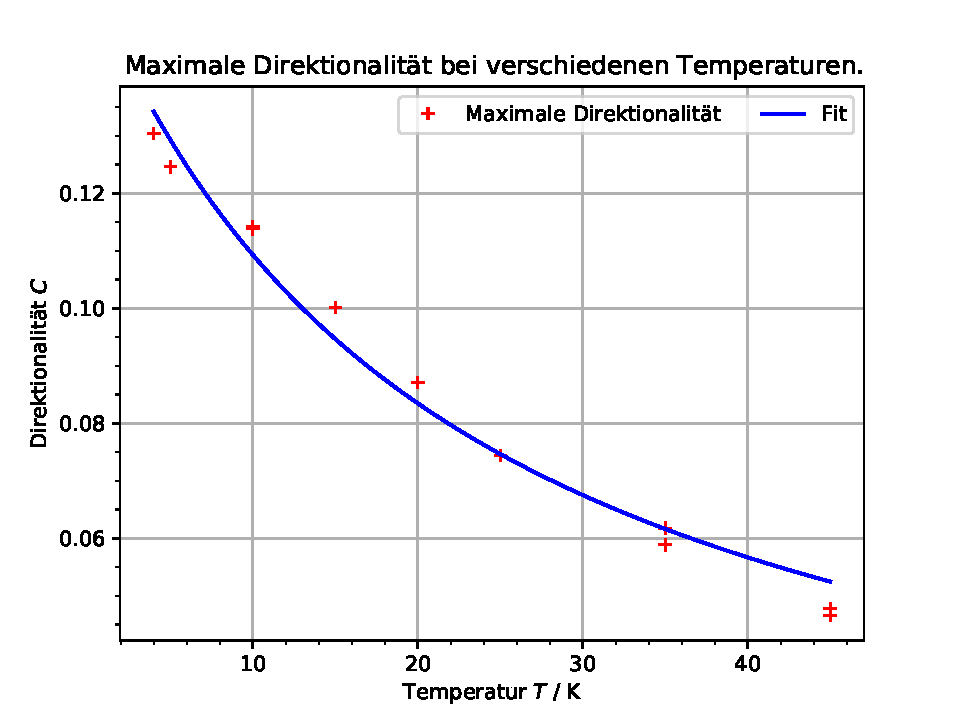
\includegraphics[scale=0.7]{./Plots/Maximale_Rho_bei_Temperaturabhänigkeit.pdf}
    \caption{Darstellung der Maximalwerte von $C$ in Abhängigkeit der Temperatur.
    Erkennbar ist die stetige Abnahme der Direktionalität $C$ bei steigender Temperatur.}
    \label{fig:fit}
\end{figure}
\FloatBarrier

Um den dargestellten Fit des Graphen zu erklären,
sind erweiternde theoretische Erläuterungen bezogen auf Abschnitt~\ref{sec:pl} notwendig.
Die im Abschnitt~\ref{sec:pl} verwendete Gleichung 
\begin{align*}
    P_c \approx \frac{2}{3} \frac{\Delta_\text{h,F}(T)}{\Delta_\text{lh}} \propto B
\end{align*}
gilt für den Bereich kleiner zirkularer Polarisation $P_{c}\ll 1$. 
Die Größe $\Delta_\text{h,F}(T)$ beschreibt die 
Zeeman-Aufspaltung der Schwerlöcher in der Faraday Geometrie.
Die Aufspaltung ist weiter definiert als~\cite{nature} 
\begin{equation}
    \Delta_\text{h,F} = xN_0\beta \bigl< S^\text{Mn}_{z} \bigr>.
\end{equation}
Dabei ist $x$ die Konzentration der $\text{Mn}^\text{2+}\text{-Ionen}$ in der Probe,
$N_0\beta = -\SI{0.88}{\eV}$ die Austauschkonstante für das Valenzband und 
$\bigl< S^\text{Mn}_{z} \bigr>$ beschreibt das thermische Mittel der Spinausrichtung
der Mn-Ionen entlang der Magnetfeldlinien des angelegten Magnetfelds.

Hierbei setzt sich $\bigl< S^\text{Mn}_{z} \bigr>$ zusammen aus~\cite{nature} 
\begin{align}
    \label{eq:S}
    \bigl< S^\text{Mn}_{z} \bigr> &= S_\text{eff} B_\text{$\frac{5}{2}$} \left(\frac{5}{2}\frac{g_\text{Mn} \mu_\text{B} B }{T_\text{eff} k_\text{B}} \right)\text{.}
    %\xi &= \frac{5}{2}\frac{g_\text{Mn} \mu_\text{B} B }{T_\text{eff} k_\text{B}}\text{,}\\
    %\label{eq:S3}
    %T_\text{eff} &= T_\text{c} + T_0\text{.} 
\end{align}
Die Größe $g_\text{Mn} = 2 $ ist der Landé-Faktor, $\mu_\text{B}$ das Bohrsche Magneton,
$k_\text{B}$ die Boltzmann-Konstante, $S_\text{eff}$ der effektive Spin und $B=\SI{0,5}{\tesla} $ das angelegte Magnetfeld.
Die effektive Temperatur $T_\text{eff}$ ist die Summe der Temperaturen $T_0$ und $T_\text{c}$.
Die Temperatur $T_\text{c}$
steht für die Temperatur des Atomgitters und $T_0$ beschreibt einen Offset, welcher durch antiferromagnetische Eigenschaften
von Mn-Paaren entsteht. Vorhergehende Experimente liefern hier einen Wert von $T_0=\SI{2}{\kelvin}$.
Die Funktion $B_{S}$ in Gleichung~\ref{eq:S} ist die Brillouin-Funktion  
\begin{equation}
    B_{S}(\xi) = \frac{2S+1}{2S}\coth\left(\frac{2S+1}{2S}\xi\right) - \frac{1}{2S}\coth(\frac{1}{2S}\xi),
\end{equation}
mit der Spinquantenzahl von $ S = \frac{5}{2}$~\cite{felix}.

Gleichung ~\ref{eq:pc} lässt sich aufgrund der Proportionalität $P_{c} \propto C(T)$~\cite{nature} 
überführen in
\begin{align}
    \label{eq:C}
    C(T)&= C_0 B_\text{$\frac{5}{2}$} \left( \frac{5}{2}\frac{g_\text{Mn} \mu_\text{B} B }{T^*_\text{eff} k_\text{B}}\right)\text{,} \\
    T^*_\text{eff} &= T + T_0 + T_\text{off}\text{.}
\end{align}
Hierbei ist $C(T)$ die Funktion die für den Fit in Abbildung~\ref{fig:fit} benutzt wird.
%
%Es gilt folgende Proportionalität~\cite{nature} 
%\begin{equation}
%    P_{c} \propto C(T). %\propto \bigl< S^\text{Mn}_{z} \bigr> 
%\end{equation}
%Die Proportionalität trifft also eine Aussage welchen Einfluss der Grad der zirkularen Polarisation $P_{c}$
%auf die Direktionalität $C(T)$ hat. 
%Je größer $P_{c}$, desto größer wird die messbare Direktionalität sein. 

Das Hauptaugenmerk im Experiment ist die Temperaturabhängigkeit von $C(T)$.
Die Temperatur beeinflusst den Grad der zirkularen Polarisation $P_c$ und das hat 
Auswirkungen auf die im Experiment ermittelbare Größe der Direktionalität $C(T)$. 
Die Temperaturabhängig von $C(T)$ besteht aus
einer modifizierten effektiven Temperatur $T^*_\text{eff}$, die aus der Summe von der gemessen Temperatur $T$, dem 
Offset $T_0$ durch die Mn-Paare (siehe oben) und dem Offset $T_\text{off}$, welches
der Temperaturdifferenz zwischen der Temperatur des Sensors und der im Experiment gemessenen entspricht. 

Die Fitparameter der Gleichung~\ref{eq:C} sind $C_0$ und $T_\text{off}$.
Diese ergeben bei der Auswertung die Werte 
\begin{align}
    C_0 & = 4,5 ± 0,3, \\
    T_\text{off} & = \SI{ 20 \pm 2}{\kelvin}.
\end{align}

Der Temperatur Offset hat mit $T_\text{off} = \SI{ 20 \pm 2}{\kelvin}$ einen sehr hohen Wert
im Vergleich zu der gemessenen Temperaturen $T$.

Der hohe Offset kommt zum einen dadurch zustande, dass sich die Probe nicht in
einen Bad aus flüssigem Helium befindet und der Temperatursensor nicht direkt
auf der Probe angebracht ist, sondern etwas weiter entfernt. 
Zum anderen, kann dieser Wert durch die Energiedichte des verwendeten Lasers von $\SI{400}{\watt\per\centi\meter^{-2}}$
erklärt werden.
Der verwendete Laser verursacht lokale Temperaturerhöhungen, welche nicht 
von dem Temperatursensor erfasst werden kann.

Durch den Verlauf des Fits in Abbildung~\ref{fig:fit} und unter der Berücksichtigung von den
vorrangestellten erweiternden theoretischen Erläuterungen wird nun klar, dass
sich die Temperaturabhängigkeit von $C(T)$ mit Hilfe von Gleichung~\ref{eq:C} in dem
gemessen Temperaturbereich gut approximieren lässt.
Um eine Verbesserung der Approximation zu erreichen, müssten weitere Temperaturmessungen 
durchgeführt werden. 
Wird der Fit und die Lage der Punkte der Direktionalität in Abbildung~\ref{fig:fit} betrachtet, so
lässt sich erahnen, dass sich wohl ein genauerer Fit mit mehr Temperaturmessungen erstellen ließe,
da die Messwerte abwechselnd um den Fit pendeln.